\documentclass[12pt]{elsarticle}
\usepackage[utf8]{inputenc}
%\usepackage{authblk}
\usepackage{setspace}
\usepackage[margin=0.75in]{geometry}
\usepackage{graphicx}
\graphicspath{ {./figures/} }
\usepackage[labelfont=bf, font = normalsize]{caption}
\usepackage{subcaption}
\usepackage{amsmath,amssymb,mathtools}
\usepackage{mathrsfs}
\usepackage{bm}
\usepackage{xcolor}
\usepackage{array}
\usepackage{appendix}
\usepackage{tikz}
\usepackage{floatrow}
\usepackage{rotating}
\usepackage{multirow,bigdelim}
\usepackage{array, blkarray, makecell}
\usepackage{tabularx}
\DeclareFloatFont{small}{\footnotesize}% "scriptsize" is defined by floatrow, "tiny" not
\floatsetup[table]{font=small}
\newcolumntype{P}[1]{>{\centering\arraybackslash}p{#1}}
\newcommand{\myparagraph}[1]{\paragraph{#1}\mbox{}\\}
\newcommand*\circled[1]{\tikz[baseline=(char.base)]{
            \node[shape=circle,draw,inner sep=2pt] (char) {#1};}}
\providecommand{\keywords}[1]
{
  \small	
  \textbf{\textit{Keywords:}} #1
}

\usepackage{siunitx}
\sisetup{per-mode = symbol}
\usepackage{tikz-3dplot}
\usepackage{graphicx}
\usetikzlibrary{calc,backgrounds}
\usepackage{pgfplotstable}
\usepgfplotslibrary{groupplots}
\usetikzlibrary{intersections}
\usetikzlibrary{positioning}
\usepgfplotslibrary{fillbetween}

%-Define RWTH colors----------------------------------------------------
\definecolor{rwth1}{RGB}{0,84,159}      % RWTH-Blau
\definecolor{rwth2}{RGB}{142,186,229}   % RWTH-Hellblau
\definecolor{rwth3}{RGB}{0,97,101}      % Petrol 
\definecolor{rwth4}{RGB}{0,152,161}     % Türkis
\definecolor{rwth5}{RGB}{87,171,39}     % Grün
\definecolor{rwth6}{RGB}{189,205,0}     % Maigrün
\definecolor{rwth7}{RGB}{255,237,0}     % Gelb
\definecolor{rwth8}{RGB}{246,168,0}     % Orange
\definecolor{rwth9}{RGB}{227,0,102}     % Magenta
\definecolor{rwth10}{RGB}{204,7,30}     % Rot
\definecolor{rwth11}{RGB}{161,16,53}    % Bordeaux
\definecolor{rwth12}{RGB}{97,33,88}     % Violett
\definecolor{rwth13}{RGB}{122,111,172}  % Lila

\definecolor{rwthb1}{HTML}{e8f1fa}      % RWTH-Blau1
\definecolor{rwthb2}{HTML}{c7ddf2}      % RWTH-Blau2
\definecolor{rwthb3}{HTML}{8ebae5}      % RWTH-Blau3
\definecolor{rwthb4}{HTML}{407fb7}      % RWTH-Blau4
\definecolor{rwthb5}{HTML}{00549f}      % RWTH-Blau5

\definecolor{rwtho1}{HTML}{fff7ea}      % RWTH-Orange1
\definecolor{rwtho2}{HTML}{feeac9}      % RWTH-Orange2
\definecolor{rwtho3}{HTML}{fdd48f}      % RWTH-Orange3
\definecolor{rwtho4}{HTML}{fabe50}      % RWTH-Orange4
\definecolor{rwtho5}{HTML}{f6a800}      % RWTH-Orange5

\definecolor{lightblue}{RGB}{173,216,230}

%-Define dash patterns--------------------------------------------------
\tikzstyle{dashpattern0} = [dash pattern = ]
\tikzstyle{dashpattern1} = [dash pattern = on 4.25pt off 0.75pt]
\tikzstyle{dashpattern2} = [dash pattern = on 1.5pt off 0.5pt]
\tikzstyle{dashpattern3} = [dash pattern = on 0.75pt off 0.4pt]
\tikzstyle{dashpattern4} = [dash pattern = on 3pt off 1pt on 1pt off 1pt]
\tikzstyle{dashpattern5} = [dash pattern = on 3.75pt off 0.5pt on 0.75pt off 0.5pt on 0.75pt off 0.5pt]
\tikzstyle{dashpattern6} = [dash pattern = on 3.25pt off 0.5pt on 0.75pt off 0.5pt on 0.75pt off 0.5pt on 0.75pt off 0.5pt]
\tikzstyle{dashpattern7} = [dash pattern = on 3.25pt off 0.5pt on 0.75pt off 0.5pt on 0.75pt off 0.5pt on 0.75pt off 0.5pt on 0.75pt off 0.5pt]
\tikzstyle{dashpattern8} = [line cap=round, dash pattern = on 3.25pt off 2.75pt]
\tikzstyle{dashpattern9} = [line cap=round, dash pattern = on 0.01pt off 2pt]
\tikzstyle{dashpattern10}= [line cap=round, dash pattern = on 3.25pt off 2pt on 0.01pt off 2pt]
\tikzstyle{dashpattern11}= [line cap=round, dash pattern = on 3.5pt off 1.75pt on 0.01pt off 1.75pt on 0.01pt off 1.75pt]
\tikzstyle{dashpattern12}= [line cap=round, dash pattern = on 3.5pt off 1.75pt on 0.01pt off 1.75pt on 0.01pt off 1.75pt on 0.01pt off 1.75pt]
\tikzstyle{dashpattern13}= [line cap=round, dash pattern = on 3.5pt off 1.75pt on 0.01pt off 1.75pt on 0.01pt off 1.75pt on 0.01pt off 1.75pt on 0.01pt off 1.75pt]

%-new commands
\newcommand{\tikzvdots}{%
  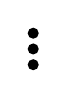
\begin{tikzpicture}[baseline=(current bounding box.center)]
    \fill (0,0) circle (2.0pt);
    \fill (0,-0.2) circle (2.0pt);
    \fill (0,-0.4) circle (2.0pt);
  \end{tikzpicture}%
}
\newcommand{\tightI}{\text{I}}
\newcommand{\tightII}{\text{I\hspace{-0.2mm}I}}
\newcommand{\tightIII}{\text{I\hspace{-0.2mm}I\hspace{-0.2mm}I}}
\newcommand{\tightIV}{\text{I\hspace{-0.2mm}V}}
            
\usepackage{tablefootnote}    
\usepackage{algorithm}
\usepackage{algpseudocode}

\usepackage{hyperref}

\usepackage{placeins}

\usepackage{amsthm}

% Define a new theorem-like environment for remarks
\newtheorem{remark}{Remark}  
            
%%%%%% Bibliography %%%%%%
% Replace "sample" in the \addbibresource line below with the name of your .bib file.

%\setcitestyle{authoryear,open={(},close={)}}
%\usepackage[style=ieee, 
%sorting=none]{biblatex}
%\setcitestyle{authoryear, open={[}, close={]}}
%\addbibresource{isrpaper.bib}

%%%%%% Title %%%%%%
% Full titles can be a maximum of 200 characters, including spaces. 
% Title Format: Use title case, capitalizing the first letter of each word, except for certain small words, such as articles and short prepositions
\usepackage{natbib}
\bibliographystyle{unsrtnat}
\title{%
	\Large A generalized dual potential for inelastic Constitutive Artificial Neural Networks: \large A JAX implementation at finite strains}

%%%%%% Authors %%%%%%
% Authors should be listed in order of contribution to the paper, by first name, then middle initial (if any), followed by last name.
% Authors should be listed in the order in which they will appear in the published version if the manuscript is accepted. 
% Use an asterisk (*) to identify the corresponding author, and be sure to include that person’s e-mail address. Use symbols (in this order: †, ‡, §, ||, ¶, #, ††, ‡‡, etc.) for author notes, such as present addresses, “These authors contributed equally to this work” notations, and similar information.

\author[1]{Hagen Holthusen \corref{cor1}}
\ead{hagen.holthusen@ifam.rwth-aachen.de}
\cortext[cor1]{Corresponding author\\hagen.holthusen@ifam.rwth-aachen.de\\ Mies-van-der-Rohe-Str. 1, 52074 Aachen, Germany}
\author[1,2]{Kevin Linka}
\author[3]{Ellen Kuhl}
\author[1]{Tim Brepols}

%%%%%% Affiliations %%%%%%
\address[1]{Institute of Applied Mechanics, RWTH Aachen University, Germany}
\address[2]{Institute for Continuum and Material Mechanics, Hamburg University of Technology, Germany}
\address[3]{Department of Mechanical Engineering, Stanford University, United States}
%\affiliation[*]{Corresponding author. Email: manjunatha@ifam.rwth-aachen.de}

%%%%%% Date %%%%%%
% Date is optional
\date{}

%%%%%% Spacing %%%%%%
% Use paragraph spacing of 1.5 or 2 (for double spacing, use command \doublespacing)
\onehalfspacing

\begin{document}

%%%%%% Abstract %%%%%%

\begin{abstract}
\begin{abstract}
Retrieval-Augmented Generation (RAG) is often used with Large Language Models (LLMs) to infuse domain knowledge or user-specific information. In RAG, given a user query, a retriever extracts chunks of relevant text from a knowledge base. These chunks are sent to an LLM as part of the input prompt. Typically, any given chunk is repeatedly retrieved across user questions. However, currently, for every question, attention-layers in LLMs fully compute the key values (KVs) repeatedly for the input chunks, as state-of-the-art methods cannot reuse KV-caches when chunks appear at arbitrary locations with arbitrary contexts. Naive reuse leads to output quality degradation.  This leads to potentially redundant computations on expensive GPUs and increases latency. In this work, we propose \sys, a system for managing and reusing precomputed KVs corresponding to the text chunks (we call \textit{chunk-caches}) in RAG-based systems. We present how to identify \hl{\textit{chunk-caches} that are reusable}, how to efficiently perform a small fraction of recomputation to \textit{fix} the cache to maintain output quality, and how to efficiently store and evict \textit{chunk-caches} in the hardware for maximizing reuse while masking any overheads. With real production workloads as well as synthetic datasets, we show that \sys reduces redundant computation by \textbf{51\%} over SOTA prefix-caching and \textbf{75\%} over full recomputation.
\hl{Additionally, with continuous batching on a real production workload, we get a \textbf{1.6$\times$} speedup in throughput and a \textbf{2$\times$} reduction in end-to-end response latency over prefix-caching while maintaining quality, for both the \llama-3-8B and \llama-3-70B models. 
}
\end{abstract}




\\
\keywords{dual potential; neural network; finite strains; generalized standard materials; inelasticity; automated model discovery} 
\end{abstract}

\maketitle

\documentclass[../main.tex]{subfiles}
\graphicspath{{../images/}}
\makeatletter
\def\input@path{{../images/}}
\makeatother
\begin{document}
\section{Introduction}
\begin{figure}
\centering
\begin{tikzpicture}
\node[inner sep=0pt] (ws) at (0, 0) {
\includegraphics[height=.4\textwidth, trim={10cm 0 10cm 0},clip]{world_space.png}};
\node[inner sep=0pt] (cs) at (6,0) {\includegraphics[height=.4\textwidth, trim={10cm 1cm 10cm 4cm},clip]{conf_space.png}};
\end{tikzpicture}
\vspace{-5pt}
\label{fig:pbrm_intro}
\caption{\textbf{Left}: Shows world space obstacles as grey spheres. Robots start and goal configuration is colored red and green, respectively. Configurations along the computed path are colored transparent blue. \textbf{Right:} Mapped world space scenario to configuration space. Obstacle region is the grey mesh. Red spheres are collision-free regions computed by the neural SCDF. The optimized shortest path in the convex corridor is the blue curve.}
\vspace{-25pt}
\end{figure}
Motion planning is the problem of finding a collision-free trajectory that connects a given start and goal configuration. The planning takes place in the configuration space of the robot. For single body robots, like mobile robots or drones, the configuration space and the world space are usually the same. This simplifies the planning, since explicit obstacle representations are available which enables geometrical tools like separating hyperplanes, smallest distance to obstacles etc., to be used when designing motion planning algorithms. For multi-body robots like manipulators, the situation is completely different. The world space obstacles are usually mapped to non-convex regions, and to make the problem even harder, the mapping is usually not known. Forming explicit representations of the obstacle region in the configuration space is usually too expensive or intractable. Despite all of this, sampling based planners are used with great success, which mainly is due to their use of implicit representations of the obstacle region. The basic idea is to construct a graph in the configuration space that covers and connects the collision-free region. From this graph, a path can be extracted that connects a given start and goal configuration. The approach is computationally expensive, since the graph is constructed with the smallest geometrical building block available, points, which represents a collision-check. Furthermore, the extracted paths from the graph are non-smooth and jagged due to the stochastic nature of the approach. This adds an additional post-processing step to the process, where the paths are shortcutted and smoothened, before the path can be used for tracking. Clearly a lot of time is invested to form this graph and produce smooth paths. Thus, if the obstacles start to move, then all of this work is done in no use, since all points that make up this graph need to be re-verified, which is simply too time consuming to be done in real time.
\\\\
In this work, we want to address the existing drawbacks of the sampling based planners. Our main contribution is an improved motion planner where each vertex in the graph covers a collision-free region in the form of a sphere instead of a point and where the edges are formed with neighboring intersecting spheres. This representation has the advantage of instead of returning piecewise linear paths, returning a sequence of overlapping spheres, i.e. a convex corridor, that connects a given start and goal configuration, illustrated in Figure \ref{fig:pbrm_intro}. This convex corridor allows us to use convex optimization to produce smooth trajectories, instead of computationally expensive post-processing methods. The representation further allows us to estimate the coverage of the collision-free space, which gives us awareness and feedback in the offline roadmap construction phase. Finally, our representation is simple to adapt to moving obstacles, simply requery for the new radii and recheck for intersections. 
\\\\
The spherical collision-free regions are formed using a signed distance function (SDF), which is a function that returns the smallest distance from an arbitrary point to the boundary of an obstacle. As the name implies, the distance is signed, thus if the point is inside the obstacle it is negative otherwise positive. If the distance is positive, a sphere with radius equal to the distance is guaranteed to cover a collision-free region. Using an SDF in motion planning is not new, but what is novel about our approach is that we express the distance in the configuration space instead of the world space and by doing so allows us to form these convex collision-free regions. We refer to the resulting SDF as a signed configuration distance function (SCDF). Computing an SCDF analytically is non-trivial, our approach is therefore to parameterize the SCDF with a deep neural network and learn the mapping by supervised learning. Our resulting neural SCDF can compute distances for different parameter values of obstacle shapes and we also show how multiple distances can be combined, thus making our approach flexible.
\section{Related work}
Motion planning algorithms can roughly be divided into three families, grid-based, sampling based and optimization based methods. Grid-based methods (GBM) discretize the planning space from which a graph is then compiled. A standard search method is A$^\star$ \citep{a_star}, which is classified as an \textit{informed} search method, since it employs a heuristic function to speed up the search. A$^\star$ guarantees to return an optimal path at the level of discretization used. GBMs usually discretize the planning space by a regular lattice and this limits the GBMs to problems with low dimensionality due to the curse of dimensionality. Thus, GBMs are usually limited to single-body robots where the degrees of freedom (DOF) are low. To overcome the inherent scaling problem with the GBMs, stochastic methods are usually used for multi-body robots. These methods are termed as sampling-based methods (SBM) and core members within this family are the rapidly-exploring random trees (RRT) \citep{rrt} and the probabilistic roadmap (PRM) \citep{prm}. RRT grows a tree from the start configuration and explores the collision-free region in a rapid way until it is able to connect to the goal region. RRT is usually improved by bi-directional planning \citep{rrt_connect}, i.e. an additional tree is grown from the goal configuration and the trees are tested for connection after any tree has been expanded. RRT is a single-query method, thus it searches for a path from scratch each time it is queried. Contrary to this, PRM is a multi-query method, which solves for multiple queries without starting from scratch. PRM does this by creating a roadmap (graph) that covers the collision-free space as an offline step. The graph is then used to solve for multiple queries. PRMs are used in cases where the environment does not change since the extra offline step is too computationally costly and needs to be re-done if the environment is changed. In our work, we address this inherent issue by using a different roadmap representation. Our vertices in the graph cover a collision-free region in the form of spheres and we form the edges by checking for intersecting spheres. If something in the environment changes, we recompute the spheres radii and recheck the intersections, without relying on collision detection. We use a trained neural network to compute the sphere radius, therefore querying for the radius can be done fast, hence our representation enables the PRM for dynamic environments.
\\\\
In the recent decades, optimization based methods (OBM) \citep{chomp, schulman, itomp, stomp} have been introduced as an alternative to SBM for multi-body robots. Like the SBM, the OBMs scale well to higher dimensional problems and produce smoother motion. It is common to use a SDF in the optimization since it is a smooth function, thus enabling gradient-based methods. However, the standard way of expressing the SDF is in world space. The distance therefore needs to be mapped to the configuration space by the forward kinematics. This mapping makes the optimization problem a non-linear program (NLP), which is computationally expensive to solve. Recently, a different approach has been proposed. In \cite{mp_gcs} motion planning is formulated as a convex optimization problem by using the graph of convex sets framework \citep{gcs}. The underlying idea is to decompose the collision-free space into intersecting convex sets from which a convex optimization problem is formulated. In cases where an explicit representation of the obstacles in the configuration space exists, like for single-body robots, creating collision-free convex regions can be done fast \citep{iris}. For multi-body robots, this is non-trivial. Existing work does this successfully \citep{iris_nlp, iris_c} by an optimization based approach, but the methods are still too time consuming to be used in the presence of moving obstacles. Our approach is instead to use deep learning to learn an SDF expressed in the configuration space. With this, we can query for shortest distances to the collision boundary, which allows us to expand spherical regions which are collision-free. Our approach is fast and therefore enables our suggested roadmap planner to be used in dynamic environments.
\\\\
Recent research has focused on learning collision detection \citep{fk_kernel_distance, diffco, graphdistnet} by predicting the signed distance between the robot links and the surrounding obstacles in the world space. The learned SDF is used in trajectory optimization but since the distance is expressed in the world space, the problem becomes an NLP and therefore takes a long time to solve. We take a novel approach and suggest to instead express the signed distance in the configuration space. This allows us to improve the PRM at the same time as it enables convex optimization for trajectory optimization, which runs faster and is more reliable than NLP solvers. In \cite{cspf} a learned signed distance function in the configuration space is proposed similar to our approach. However, their approach is restricted to point cloud representations, while we propose to represent the obstacles as parameterized geometric shapes, e.g. spheres. Furthermore, we also show how to use our learned SCDF to improve an existing roadmap planner.
\section{Problem formulation}
A robot is located in the world space, $\W \subset \R^3 $. The unique location of the robot is given by its configuration $\q \in \C$, where $\C$ is the configuration space. The set of points covered by the robots bodies at a certain configuration is expressed as $\B(\q) \subset \W$. The robot is surrounded by $\NrObst$ obstacles $\O = \bigcup_{i=1}^{\NrObst} \O_i$, where  $\O_i \subset \W$. The representation of the obstacle in the configuration space is the set $\C\O_i = \{\q \in \C \: |\: \B(\q) \cap \O_i \neq \emptyset \}$. The obstacle space is formed as $\Co = \bigcup_{i=1}^{\NrObst} \C \O_i$. The complement is referred to as the free space, $\Cf = \C \setminus \Co$. The path planning problem is a tuple, ($\Cf$, $\qStart$, $\qGoal$), where we want to connect a query pair, consisting of a start, $\qStart$, and goal configuration, $\qGoal$, with a geometric path, $\q(s): [0, 1] \mapsto \Cf$, such that $\q(0)=\qStart$ and $\q(1)=\qGoal$, or report correctly when such a path does not exist.
\end{document}

\section{Constitutive framework for finite strain inelasticity}
\label{sec:constitutive}
%
In this section, we briefly outline the underlying constitutive framework for general inelastic materials at finite strains, which are modeled using the multiplicative decomposition of the deformation gradient.
For this, we introduce two fundamental scalar-valued quantities: 
The Helmholtz free energy, $\psi$, as well as a dual potential, $\omega$.
All constitutively dependent quantities can be derived from these thermodynamic potentials.
This dual potential approach is certainly not the only method for modeling inelastic behavior. We will elucidate its close relationship to Generalized Standard Materials \cite{halphen1975}, another well-established framework for characterizing inelasticity, in Section~\ref{sec:GSM}.\newline

\textbf{Kinematics.} We employ the multiplicative decomposition of the deformation gradient, $\bm{F}=\bm{F}_e\bm{F}_i$, into an elastic part, $\bm{F}_e$, and an inelastic part, $\bm{F}_i$, cf. \cite{Eckart1948,Kroener1959,sidoroff1974,rodriguez1994}.
Both determinants of the individual parts are greater than zero.
Conceptually, we introduce an intermediate configuration, relative to which the elastic response is characterized.
Unfortunately, the multiplicative decomposition is non-unique, i.e.\ we may superimpose any rotation $\bm{F}=\bm{F}_e\bm{Q}^{\dagger^T}\bm{Q}^\dagger\bm{F}_i=:\bm{F}_e^\dagger\bm{F}_i^\dagger$ where $\bm{Q}^\dagger \in \mathrm{SO}(3)$ with $\mathrm{SO}(3)$ denoting the special orthogonal group.
By employing the singular value decomposition, we recognize that $\bm{F}_i$ and $\bm{F}_i^\dagger$ share the same singular values, and thus, the same stretch tensor $\bm{U}_i$ resulting from the polar decomposition $\bm{F}_i=\bm{R}_i\bm{U}_i$ with $\bm{R}_i \in \mathrm{SO}(3)$.
Thus, we find $\bm{U}_i$ to be unique, and further, $\bm{F}_i^\dagger=\bm{R}_i^\dagger\bm{U}_i$ where $\bm{R}_i^\dagger=\bm{Q}^\dagger\bm{R}_i$.
Lastly, we introduce an appropriate stretch measure of the elastic stretches $\bm{C}_e = \bm{F}_e^T\bm{F}_e = \bm{Q}^\dagger\bm{F}_e^{\dagger^T}\bm{F}_e^\dagger\bm{Q}^{\dagger^T}$, which however, is non-unique.\newline

\textbf{Clausius-Planck inequality.} Any constitutive framework for solids must satisfy the Clausius-Planck inequality $\mathcal{D} := -\dot{\psi} + 1/2\, \bm{S}:\dot{\bm{C}} \geq 0$ where $\bm{S}$ denotes the second Piola-Kirchhoff stress, while $\bm{C}=\bm{F}^T\bm{F}$ refers to the right Cauchy-Green tensor.
For the time being, we assume the Helmholtz free energy to be a scalar-valued isotropic function \cite{spencer1971,zheng1994} depending solely on $\bm{C}_e$, i.e. $\psi = \hat{\psi}(\bm{C}_e)$.
Hence, we obtain the following, cf. \cite{dettmer2004}
%
\begin{equation}
\mathcal{D} =    \left(\bm{S} - 2\,\bm{F}_i^{-1}\,\frac{\partial\psi}{\partial\bm{C}_e}\,\bm{F}_i^{-T} \right) : \frac{1}{2}\,\dot{\bm{C}} + \underbrace{2\,\bm{C}_e\,\frac{\partial\psi}{\partial\bm{C}_e}}_{=: \bm{\Sigma}} : \underbrace{\dot{\bm{F}}_i\bm{F}_i^{-1}}_{=: \bm{L}_i} \geq 0
\label{eq:dissipation}
\end{equation}
%
where we introduce the elastic Mandel-like stress $\bm{\Sigma}$, which is symmetric since $\psi$ is an isotropic function of $\bm{C}_e$, cf. \cite{svendsen2001}\footnote{In the case of initial anisotropy, $\psi$ is usually assumed to be an isotropic function of $\bm{C}_e$ and a structural tensor $\bm{H}$. Note that in this case $\bm{\Sigma}$ is no longer symmetric.}.
Noteworthy, since $\bm{\Sigma}$ solely depends on $\bm{C}_e$, the elastic Mandel-like stress is also non-unique, i.e. $\bm{\Sigma}=\bm{Q}^{\dagger}\bm{\Sigma}^\dagger\bm{Q}^{\dagger^T}$.
Following the arguments of \cite{coleman1961,coleman1963,coleman1967}, we assume the term in brackets in Inequality~\eqref{eq:dissipation} to be zero, revealing the state law for $\bm{S}$.
Consequently, as $\bm{\Sigma}$ is symmetric, we can reduce the dissipation inequality to
%
\begin{equation}
    \mathcal{D}_{red} := \bm{\Sigma} : \bm{D}_i \geq 0
    \label{eq:dissipation_red}
\end{equation}
%
where $\bm{D}_i := \mathrm{sym}(\bm{L}_i)$ is the symmetric part of $\bm{L}_i$.
To satisfy the reduced dissipation inequality for arbitrary processes, we will introduce a dual potential, $\omega=\hat{\omega}(\bm{\Sigma})$, which is assumed to be a scalar-valued isotropic function in order to be independent of the superimposed rotation $\bm{Q}^\dagger$.\newline

\textbf{Co-rotated intermediate configuration.} We have observed that the relevant constitutive quantities, such as $\bm{C}_e$ and $\bm{\Sigma}$, suffer from an inherent rotational non-uniqueness.
This poses challenges in computing these quantities and derivatives with respect to those, for instance $\frac{\partial\psi}{\partial\bm{C}_e}$.
To address this issue in our numerical implementation, we adopt the approach suggested by \cite{holthusen2023} and introduce a co-rotated intermediate configuration.
In short, this approach pulls all non-unique quantities back by either $\bm{R}_i$ or $\bm{R}_i^\dagger$, i.e. $\bar{(\bullet)}:=\bm{R}_i^T\,(\bullet)\,\bm{R}_i = \bm{R}_i^{\dagger^T}\,(\bullet)^\dagger\,\bm{R}_i^\dagger$.
Consequently, we obtain the following unique quantities
%
\begin{equation}
    \label{tb_eq:10}
    \bar{\bm{C}}_e = \bm{U}_i^{-1}\bm{C}\bm{U}_i^{-1}, \quad \bm{S} = 2\,\bm{U}_i^{-1}\,\frac{\partial\psi}{\partial\bar{\bm{C}}_e}\,\bm{U}_i^{-1}, \quad \bar{\bm{\Sigma}} = 2\,\bar{\bm{C}}_e\,\frac{\partial\psi}{\partial\bar{\bm{C}}_e}, \quad \bar{\bm{D}}_i = \mathrm{sym}\left(\dot{\bm{U}}_i\,\bm{U}_i^{-1} \right).
\end{equation}
%
Noteworthy, the co-rotated pullback preserves both the symmetry as well as the eigenvalues, which is considered an advantage.\newline

\textbf{Potential-based evolution equation.} It remains to introduce an evolution equation for $\bar{\bm{D}}_i$ in a thermodynamic consistent way such that Inequality~\eqref{eq:dissipation_red} is satisfied for arbitrary processes.
Therefore, we postulate the existence of a pseudo potential \cite{kerstin1969}, which we may identify as the dual potential resulting from the Legendre-Fenchel transformation of the `classical' dissipation potential (see Section~\ref{sec:GSM}) known from Generalized Standard Materials \cite{halphen1975}, viz.\
%
\begin{equation}
    \bar{\bm{D}}_i = \frac{\partial \omega\left(\bar{\bm{\Sigma}}\right)}{\partial\bar{\bm{\Sigma}}}.
\label{eq:EvolutionEquation}
\end{equation}
%
According to \citet{germain1983}, the dissipation inequality is naturally fulfilled if $\omega$ is \textit{convex}, \textit{zero-valued}, and \textit{non-negative} with respect to $\bar{\bm{\Sigma}}$ \cite{holthusen2025growth}\footnote{We may understand the evolution equation as a subderivative $\bar{\bm{D}}_i \in \partial_{\bar{\bm{\Sigma}}}\omega\left(\bar{\bm{\Sigma}}\right)$ in case of non-smooth potentials, where $\partial_{\bar{\bm{\Sigma}}}\omega\left(\bar{\bm{\Sigma}}\right)$ denotes the subderivative with respect to $\bar{\bm{\Sigma}}$, see \cite{germain1998}.}.\newline

\textbf{Invariant representation.} As discussed above, the dual potential is assumed to be an isotropic function of $\bar{\bm{\Sigma}}$, and can, thus, be expressed in terms of its invariants.
Here, we choose the common stress invariants $I_1^{\bar{\bm{\Sigma}}}:=\mathrm{tr}(\bar{\bm{\Sigma}})$, $J_2^{\bar{\bm{\Sigma}}}:=1/2\,\mathrm{tr}(\mathrm{dev}(\bar{\bm{\Sigma}})^2)$, and $J_3^{\bar{\bm{\Sigma}}}:=1/3\,\mathrm{tr}(\mathrm{dev}(\bar{\bm{\Sigma}})^3)$.
With these invariants at hand, the evolution equation reduces to
%
\begin{equation}
    \bar{\bm{D}}_i = \frac{\partial\omega^*}{\partial\bar{\bm{\Sigma}}} = \frac{\partial\omega^*}{\partial I_1^{\bar{\bm{\Sigma}}}}\,\bm{I} + \frac{\partial\omega^*}{\partial J_2^{\bar{\bm{\Sigma}}}}\,\mathrm{dev}\left(\bar{\bm{\Sigma}}\right) + \frac{\partial\omega^*}{\partial J_3^{\bar{\bm{\Sigma}}}}\,\mathrm{dev}\left(\mathrm{dev}\left(\bar{\bm{\Sigma}}\right)^2\right)
\label{eq:EvolutionEquationInvars}
\end{equation}
%
where $\omega^*=\hat{\omega}^*\left(I_1^{\bar{\bm{\Sigma}}},\sqrt{J_2^{\bar{\bm{\Sigma}}}},\sqrt[3]{J_3^{\bar{\bm{\Sigma}}}}\right)$.
The square and cubic roots are calculated to ensure that all invariants share the same unit.
If we plug \eqref{eq:EvolutionEquationInvars} into the co-rotated version of Equation~\eqref{eq:dissipation_red}
%
\begin{equation}
    %\mathcal{D}_{red} := \frac{\partial\omega^*}{\partial I_1^{\bar{\bm{\Sigma}}}}\,I_1^{\bar{\bm{\Sigma}}} + \frac{\partial\omega^*}{\partial \sqrt{J_2^{\bar{\bm{\Sigma}}}}}\,\sqrt{J_2^{\bar{\bm{\Sigma}}}} + \frac{\partial\omega^*}{\partial \sqrt[3]{J_3^{\bar{\bm{\Sigma}}}}}\,\sqrt[3]{J_3^{\bar{\bm{\Sigma}}}} \geq 0,
    \mathcal{D}_{red} = \nabla\omega^*(\mathbf{z}) \cdot \mathbf{z} \geq 0, \quad \mathbf{z} = \begin{pmatrix}
        I_1^{\bar{\bm{\Sigma}}} \\
        \sqrt{J_2^{\bar{\bm{\Sigma}}}} \\
        \sqrt[3]{J_3^{\bar{\bm{\Sigma}}}}
    \end{pmatrix}
    \label{eq:reduced_dissipation_vector}
\end{equation}
%
we observe that the inequality is satisfied if $\omega^*$ is convex, zero-valued, and non-negative with respect to its arguments; however, this does not guarantee its convexity with respect to $\bar{\bm{\Sigma}}$, cf. \cite{collins2002}.
The reason for this lies in the indefinite Hessian of $J_3^{\bar{\bm{\Sigma}}}$ with respect to the Mandel-like stress.
Nevertheless, non-convex yield surfaces, which are typically modelled as a potential subtracted by a threshold such as the yield stress, are not only of significant practical relevance \cite{gluege2017,matzenmiller1995,baghous2022} but also amenable to numerical treatment \cite{sheng2011,pedroso2008}.
As $\omega^*$ includes the special case of being convex with respect to $\bar{\bm{\Sigma}}$, we consider this framework advantageous. 
%
%=================================
\subsection{Relation to Generalized Standard Materials for solids}
\label{sec:GSM}
In the following, we will explain the intrinsic relationship between the present modeling framework for iCANNs and the classical framework of Generalized Standard Materials, the latter of which is well-known in the literature (see e.g.\ \cite{halphen1975,germain1983,flaschel2023}). We start again with the Helmholtz free energy and assume, for the same reasons as explained above, that it is a scalar-valued isotropic function of quantities in the co-rotated intermediate configuration. Specifically, we assume a dependence of $\psi$ on $\bar{\bm{C}}_e$ only, i.e.\ $\psi = \hat{\psi}(\bar{\bm{C}}_e)$. More general cases in which $\psi$ additionally depends on further internal state variables or structural tensors are, of course, possible. However, since this does not lead to additional insights in the presentation that follows, we will not consider this case for simplicity.

Exploiting again the Clausius-Planck inequality and the chain rule of differentiation, we may arrive at
\begin{equation}
\label{tb_eq:1}
\mathcal{D} = -\dot{\psi} + \frac{1}{2}\, \bm{S}:\dot{\bm{C}} \geq 0 \qquad \Rightarrow \qquad \mathcal{D} = -2\,\frac{\partial \psi}{\partial \bar{\bm{C}}_e} : \frac{1}{2}\,\dot{\bar{\bm{C}}}_e + \bm{S}:\frac{1}{2}\,\dot{\bm{C}} \geq 0.
\end{equation}
Considering $\bar{\bm{C}}_e = \bm{U}_i^{-1}\,\bm{C}\,\bm{U}_i^{-1}$, the relation $\dot{\bm{C}} = \dot{\bm{U}}_i\,\bar{\bm{C}}_e\,\bm{U}_i + \bm{U}_i\,\dot{\bar{\bm{C}}}_e\,\bm{U}_i + \bm{U}_i\,\bar{\bm{C}}_e\,\dot{\bm{U}}_i$, and well-known properties of the scalar product of two second-order tensors, Inequality~\eqref{tb_eq:1} can directly be rewritten as
\begin{equation}
\label{tb_eq:2}
\mathcal{D} = \left(\bar{\bm{S}} - 2\,\frac{\partial \psi}{\partial \bar{\bm{C}}_e}\right):\frac{1}{2}\,\dot{\bar{\bm{C}}}_e + \bar{\bm{\Sigma}}:\bar{\bm{L}}_i \geq 0.
\end{equation}
Here, $\bar{\bm{S}} := \bm{U}_i\,\bm{S}\,\bm{U}_i$ is the second Piola–Kirchhoff stress tensor relative to the co-rotated intermediate configuration and $\bar{\bm{\Sigma}} = \bar{\bm{C}}_e\,\bar{\bm{S}}$ denotes the (up to this point generally unsymmetric) Mandel-like stress tensor in the very same configuration. With $\bar{\bm{L}}_i = \mathrm{sym}(\bar{\bm{L}}_i) + \mathrm{skew}(\bar{\bm{L}}_i) = \bar{\bm{D}}_i + \bar{\bm{W}}_i$, Expression~\eqref{tb_eq:2} is finally rewritten as
\begin{equation}
\label{tb_eq:3}
\mathcal{D} = \bar{\bm{S}}^{\,\mathrm{dis}}:\frac{1}{2}\,\dot{\bar{\bm{C}}}_e + \mathrm{sym}(\bar{\bm{\Sigma}}):\bar{\bm{D}}_i + \mathrm{skew}(\bar{\bm{\Sigma}}):\bar{\bm{W}}_i \geq 0
\end{equation}
where $\bar{\bm{S}}^{\,\mathrm{dis}} := \left(\bar{\bm{S}} - 2\,\frac{\partial \psi}{\partial \bar{\bm{C}}_e}\right)$ can be considered the irreversible or dissipative part of the stress $\bar{\bm{S}}$.

To fulfill dissipation inequality~\eqref{tb_eq:3}, it is now customary in the framework of Generalized Standard Materials to assume a scalar-valued dissipation potential\footnote{As in case of the Helmholtz free energy $\psi$, we may directly formulate the dissipation potential $\Omega$ as a scalar-valued isotropic function of quantities in the co-rotated intermediate configuration, in order to avoid any ambiguities due to arbitrary rotations of the intermediate configuration.} $\Omega = \hat{\Omega}\left(\dot{\bar{\bm{C}}}_e,\bar{\bm{D}}_i,\bar{\bm{W}}_i\right)$, expressed in terms of the strain-like rate quantities $\dot{\bar{\bm{C}}}_e$, $\bar{\bm{D}}_i$, and $\bar{\bm{W}}_i$, which is convex, non-negative, and zero-valued at the origin, i.e.\ $\hat{\Omega}(\bm{0},\bm{0},\bm{0}) = 0$. This potential is conveniently used to derive complementary laws for the thermodynamic conjugate forces, i.e.\footnote{In case of a non-smooth dissipation potential $\Omega$, the partial derivatives in \eqref{tb_eq:4} and the following should be understood as subderivatives.}:
\begin{equation}
\label{tb_eq:4}
\bar{\bm{S}}^{\,\mathrm{dis}} = \frac{\partial \Omega}{\partial \dot{\bar{\bm{C}}}_e}, \qquad \mathrm{sym}(\bar{\bm{\Sigma}}) = \frac{\partial \Omega}{\partial \bar{\bm{D}}_i}, \qquad \mathrm{skew}(\bar{\bm{\Sigma}}) = \frac{\partial \Omega}{\partial \bar{\bm{W}}_i}.
\end{equation}
As can be shown, with the above definitions, thermodynamic consistency of the formulation is naturally ensured.\newline

\textbf{Strain-rate independent dissipation potential.} Further consequences for the dissipation potential arise when dealing with solid materials, for which it is usually assumed that purely elastic, but otherwise arbitrary deformations ($\dot{\bar{\bm{C}}}_e \ne \bm{0}$, $\bar{\bm{D}}_i = \bar{\bm{W}}_i = \bm{0}$) do not cause any dissipation. In this case, it can be inferred from Inequality \eqref{tb_eq:3} that
\begin{equation}
\label{tb_eq:5}
\mathcal{D} = \bar{\bm{S}}^{\,\mathrm{dis}}:\frac{1}{2}\,\dot{\bar{\bm{C}}}_e = 0 \qquad \Rightarrow \qquad \bar{\bm{S}}^{\,\mathrm{dis}} = \frac{\partial \hat{\Omega}}{\partial \dot{\bar{\bm{C}}}_e} = \bm{0}.
\end{equation}
In other words, it can be concluded that the dissipation potential cannot be a function of the elastic strain rate $\dot{\bar{\bm{C}}}_e$ in this case\footnote{This does by no means preclude any strain-rate-dependent behavior of the material model, as the rate dependency can be reflected in the evolution of the internal state variables.}. Furthermore, as the second Piola-Kirchoff stress tensor relative to the intermediate configuration becomes $\bar{\bm{S}} = 2\,\frac{\partial \psi}{\partial \bar{\bm{C}}_e}$, this immediately leads to a symmetric Mandel-like stress tensor $\bar{\bm{\Sigma}} = \bar{\bm{C}}_e\,\bar{\bm{S}} =  2\,\bar{\bm{C}}_e\,\frac{\partial\psi}{\partial\bar{\bm{C}}_e}$ (see also \eqref{tb_eq:10}$_3$), i.e.\ $ \mathrm{sym}(\bar{\bm{\Sigma}}) = \bar{\bm{\Sigma}}$ and $\mathrm{skew}(\bar{\bm{\Sigma}}) = \bm{0}$. The Clausius-Planck inequality therefore reduces to 
\begin{equation}
\label{tb_eq:6}
\mathcal{D}_{red} = \bar{\bm{\Sigma}}:\bar{\bm{D}}_i\geq 0,
\end{equation}
such that the dissipation potential needs to be a function of $\bar{\bm{D}}_i$ only, i.e.\ $\Omega = \hat{\Omega}(\bar{\bm{D}}_i)$ with $\hat{\Omega}(\bm{0}) = 0$. The complementary law for $\bar{\bm{\Sigma}}$ is then obtained as
\begin{equation}
\label{tb_eq:11}
\bar{\bm{\Sigma}} = \frac{\partial \Omega}{\partial \bar{\bm{D}}_i}.
\end{equation}

\textbf{Dual dissipation potential in terms of stress-like quantities.}
Finally, by means of a Legendre-Fenchel transformation of $\Omega$, a dual dissipation potential $\omega$ in terms of the stress-like quantity $\bar{\bm{\Sigma}}$ can be derived:
\begin{equation}
\label{tb_eq:8}
    \omega = \hat{\omega}(\bar{\bm{\Sigma}}) = \sup_{\bar{\bm{D}}_i}\left(\bar{\bm{\Sigma}} : \bar{\bm{D}}_i - \hat{\Omega}\!\left(\bar{\bm{D}}_i\right)\right).
\end{equation}
The latter potential is also convex, non-negative, and zero-valued at the origin, i.e.\ $\hat{\omega}(\bm{0}) = 0$. It can be employed to define a thermodynamically consistent evolution equation (or complementary law) for the strain-like internal state variable $\bar{\bm{D}}_i$ via
\begin{equation}
\label{tb_eq:11}
    \bar{\bm{D}}_i = \frac{\partial \omega}{\partial \bar{\bm{\Sigma}}}.
\end{equation}

\textbf{Relation to iCANN framework.} The above shows that iCANNs perfectly fit into the framework of Generalized Standard Materials. The only difference to the more classical approach is that, in the iCANN modeling framework presented here, the dual dissipation potential \eqref{tb_eq:8} in terms of the stress-like variable $\bar{\bm{\Sigma}}$ is constructed and identified \emph{directly}. However, this alternative procedure is by no means unusual or disadvantageous, and has been proposed as an equally valid approach by other authors in the past (among many others, \cite{LemaitreChaboche1994,Chaboche1997,LeuschnerFritzenEtAl2015,HoltzmanChrysochoosEtAl2018}). One potential can always be constructed from the other, owing to the remarkable duality of the Legendre-Fenchel transformation. 
\section{Network Issues} \label{sec:network-issues}
This section delves into the network layer's vulnerabilities, pivotal for synchronizing time across digital systems. Such synchronization is vital for applications ranging from digital payments to industrial automation. Yet, it faces threats from \textit{attackers controlling network devices} (on-path attacker) or \textit{possessing privileged access to a victim's local network stack} (off-path attacker).

\subsection{Limited Use of Authentication Mechanisms} Cryptography techniques, used by protocols like NTP~\cite{ntpv4-rfc} and PTP~\cite{ptp-std-doc}, play a critical role in ensuring data integrity and origin authentication of the time-sync traffic, thwarting man-in-the-middle (MITM) attacks. Yet, several issues persist regarding the adoption of these methods making time-sync protocols vulnerable to attacks.


\noindent\textbf{\texttt{I10.} False packet injection.} A MITM adversary can impersonate a genuine time server and send false time-sync packets to the target. These attacks may result from weak assumptions underlying the authentication mechanism adopted by the time-sync protocol. For instance, the reliance of NTP's broadcast mode authentication protocol TESLA~\cite{tesla-cryptography} (also used by PTP~\cite{ptp-std-doc}) on loosely synchronized devices creates a circular dependency between authentication and time-sync~\cite{ntp-replay-drop-attack}, rendering the former useless. Moreover, infiltration of malicious servers in the pool of legitimate time servers is  a genuine concern~\cite{shark-ntp-pool, devil-time-origin}. It is because cryptographic authentication only protects against a MITM attacker and the malicious servers render it ineffective. This allows Kwon et. al., to use a handful of malicious time servers, injected to the NTP pool~\cite{ntpd-pool-project}, to disrupt time-sync clients spread over entire countries~\cite{shark-ntp-pool}. Despite their shortcomings, authentication techniques make packet injection attacks harder. However, the adoption of these mechanisms is not universal. For instance, Huygens~\cite{huygens}, RBS~\cite{Elson2003RBS}, FTSP~\cite{ftsp-2004}, TPSN~\cite{tpsn-2003} do not implement any origin authentication mechanisms and have no protection against packet injection. The severity of the issue is evident from the fact that \textit{RBS, FTSP and TPSN} are among the most cited protocols for time-sync in sensor networks. In contrast, secure time synchronization protocols such as the one introduced by Ganeriwal et. al.~\cite{net-sync-wsn-sec-prot} has received an order of magnitude fewer citations (see table~\ref{tab:time-sync-wsn-citations}). Packet injection is one of the most potent attacks against time-sync protocols and could be used to induce \textit{time travel, warping or just increased uncertainty} (\textbf{\texttt{A1-3}}) in the victim's view of time.

\begin{table}
\scriptsize
\centering
\begin{tabular}{ | c | c | c | c | }
 \hline
  \textbf{Protocol} & \textbf{Authentication} & \textbf{Date Published} & \textbf{Citations} \\
 \hline
 \hline
  RBS~\cite{Elson2003RBS}  & \textit{No} & $2003$ & $3927$   \\
 \hline
   TPSN~\cite{tpsn-2003}  & \textit{No} & $2003$ & $3206$   \\
 \hline
   FTSP~\cite{ftsp-2004}  & \textit{No} & $2004$ & $3052$   \\
 \hline
 \hline
   Secure Time-Sync~\cite{Elson2003RBS}  & \textit{Yes} & $2005$ & $278$   \\
 \hline
\end{tabular}
\caption{One of the earliest time-sync protocols proposed for wireless sensor networks (WSNs). The protocols (RBS, TPSN and FTSP) that do not incorporate authentication mechanisms have received an order of magnitude more citations than the protocol (STS) that make use of cryptography mechanisms. \textit{Source: Google Scholars as of Jan 22, 2024.}}
\label{tab:time-sync-wsn-citations}
\end{table}

\noindent\textbf{\texttt{I11.} Packet modification.} Correct implementation of authentication protocols prevents false packet injection but may not prevent against packet modification. This is best exemplified by PTP, which makes use of authentication~\cite{ptp-std-doc} to protects the PTP packets except the correction field of the packet header. This field allows each network node to update correction field with the packet processing delay. PTP uses this information to achieve better time-sync accuracy by eliminating the variable network delays~\cite{net-sync-ptp-covert-channel}. However, a MITM attacker (on-path or off-path) can add incorrect information to this field and manipulate the PTP client. Jacobs et, al., use this channel to introduce \textit{significant offsets} (\textbf{\texttt{A3}}) to the victim device while \textit{avoiding detection}. They could also induce the victim device to change its clock frequency (\textbf{\textit{A2}}), resulting in an even larger time deviation from the time server~\cite{net-sync-ptp-covert-channel}. We note that this attack is not PTP specific, and any time-sync protocol seeking network delay information may be subject to this attack. Finally, we also note that this technique is less sophisticated as it does not require by-passing authentication requires.

\noindent\textbf{\texttt{I12.} Packet replay.} Authentication issues discussed in $I10$ can also result in replay attacks. In this attack, the adversary repeatedly sends one or a sequence of pre-recorded time server packets to the victim. Packet replay attacks have been successfully demonstrated against NTP broadcast mode~\cite{ntp-replay-drop-attack}. Malhotra et. al. exploited limitations in existing NTP client implementations to keep the victim stuck at a single point in time (\textbf{\texttt{A1}}). They point out that the one-way nature of the time-sync traffic (NTP broadcast mode) enables this attack. It implies that other one-way time synchronization protocols such as RBS~\cite{Elson2003RBS} may also be susceptible to this attack.

\noindent\textbf{\texttt{I13.} Spoofing Wireless Timing Signals.} Time-sync protocols like GPS, ROCS~\cite{ROCS-FM-Beacons}, Syntonizor~\cite{Syntonizor-AC-powerlines} and WizSync~\cite{WizSync-Wifi-Beacons} work using a periodic wireless timing signal that is transmitted directly from the timing source(s) to the clients i.e. over a single hop. These protocols lack authentication mechanisms allowing adversaries to spoof timing signals. This attack is the equivalent to packet manipulation attack on packet exchange based protocols (NTP~\cite{nts-rfc}, PTP~\cite{ptp-std-doc}, FTSP~\cite{ftsp-2004} etc.). Similar to the packet manipulation attacks, an external adversary mimics a trusted timing source but transmits incorrect timing information. It does so by generating a powerful spoof signal, using antenna(s), that can overpower the legitimate signal. Such an attacker often stays \textit{stealthy} while introducing uncertainty in the victim's local clocks~\cite{gps-spoofing-fundamentals} (\textbf{\texttt{A3}}). Satellite based global positing systems (GPS) is a typical target of this attack~\cite{gps-spoofing-21}. However, other time-sync protocols in this category (e.g., ROCS,~\cite{ROCS-FM-Beacons}, WizSync~\cite{WizSync-Wifi-Beacons} and Syntonizor~\cite{Syntonizor-AC-powerlines} etc.) haven't seen significant spoofing attacks due to their limited application. Nevertheless, signal spoofing remains a viable attack option for a motivated adversary.

\subsection{Availability Issues}
Beyond modifying timing packets, time-sync is also affected by just delaying the transmission of the timing information (as discussed in section~\ref{subsec:case-studies}). An adversary may leverage this observation and use unpredictable delays to add errors to the time-sync process or it  may outright block time-sync traffic headed towards the victim. 

\noindent\textbf{\texttt{I14.} Packet delay.} Time synchronization protocols determine the time offset between the server and the client by exchanging packets over the network. These network packets experience delays causing uncertainty in the exchanged timing information and the corresponding offset calculations (see section~\ref{subsec:case-studies}). Time-sync protocols rely heavily on precise network delay measurements to remove this uncertainty in the offset estimations. NTP~\cite{ntpv4-rfc} solves this challenge by measuring round trip times (RTTs) and computes network delay as half of the RTT, assuming symmetric delays~\cite{rfc1305}. On the other hand PTP measures the network delays by mandating each processing node to update the PTP packets with its resident delay (see $I11$). While effective under normal network conditions, these delay estimation mechanisms are not robust to adversarial delays. A malicious network node may introduce additional network delays~\footnote{In case of NTP, the server-bound and client-bound packets are delayed by different duration while for PTP the adversary would not update PTP packets with its resident delay} to degrade the synchronization performance. For instance, Annesi et. al. show that delay attacks against PTP can induce errors of several milliseconds, accumulating over time to even larger values under a sustained attacks~\cite{ptp-futile-encryption} (\textbf{\texttt{A2}}). However, vulnerability to delay attacks extend beyond NTP and PTP; virtually all time-sync protocols are susceptible to these attacks.

\noindent\textbf{\texttt{I15.} Packet drop.} 
Intercepting and dropping time-sync packets is a simple yet effective MiTM attack that desynchronizes the victim device from its time server. Facing this \textit{denial-of-service} attack, the victim solely relies on its \textit{local clock} which diverges away from the server time (\textbf{\texttt{A3}}) dictated by the stability of the victim's time source. For low-end systems using inexpensive quartz crystals, the time difference may accumulate to several minutes per day. In contrast, devices using more stable oven-controlled quartz oscillators may experience deviations of only a few seconds in the same period. However, despite its effectiveness, the victim can deduce potential instances of this attack, with relative ease, from sudden unavailability of time-server.

\noindent\textbf{\texttt{I16.} Blocking Wireless Timing Signals.} For single-hop wireless time synchronization (GPS~\cite{gps-spoofing-fundamentals}, ROCS~\cite{ROCS-FM-Beacons}, WizSync~\cite{WizSync-Wifi-Beacons} etc.), denial of service attack takes the form of blocking the wireless timing signal. An adversary achieves this by generating high powered noise in the frequency band used by the wireless timing signal. It requires physical proximity to the target and signal transmission equipment, raising the cost of this attack. Nevertheless, GPS signal blocking techniques have been studied extensively~\cite{gps-jamming-overview} due to ubiquitous use of GPS by defense and civil infrastructure. In principle, other single-hop wireless protocols such as Syntonizor~\cite{Syntonizor-AC-powerlines} and ROC~\cite{ROCS-FM-Beacons} are also vulnerable to these attacks, even though no such attack against them is known.

\subsection{Implementation Issues} In addition to the the communication medium, the end-points of this channel i.e. the applications implementing the time-sync protocol themselves represent an attack surface.

\noindent\textbf{\texttt{I17.} Untrusted time synchronization software.} Applications implementing time-sync protocols may harbor security vulnerabilities of their own. For instance, CVE database lists 98 vulnerabilities, discovered over the years, in the NTP application developed by \textit{NTP.org}~\cite{ntp-cve-details}. This application is used by both the time-sync clients and servers,~\footnote{It is recommended for servers joining the NTP pool project~\cite{ntpd-pool-project}.} and can be exploited by an adversary with access to \textit{privileged execution} on the victim device or \textit{a network connection to the NTP application}. An attack exploiting client side application vulnerability would only affect a single machine, however, the server side exploit would affect time alignment at all of its clients. Further, these attacks may cause the target applications to crash pausing the time-sync service or may just degrade time-sync performance (\textbf{\texttt{A3}}) over longer periods. It is worth pointing out time-sync applications executing in the privileged context present an even bigger risk, as any vulnerability in them could compromise the system beyond time-sync service.
\begin{table}[ht!]
\centering
\caption{\textbf{Super Resolution Performance Results.} Our proposed WGAN EEG Spatial Upsampling method significantly outperforms a baseline of Bicubic Interpolation commonly used in EEG upsampling pipelines.}
\label{tab:results}
\resizebox{0.8\linewidth}{!}{%
\begin{tabular}{@{}cccccc@{}}
\toprule
\multirow{2}{*}{\textbf{Dataset}} & \multirow{2}{*}{\textbf{Scale}} & \multicolumn{2}{c}{\textbf{Bicubic}} & \multicolumn{2}{c}{\textbf{WGAN}} \\ \cmidrule(l){3-6} 
                      &   & \textbf{MSE} & \textbf{MAE} & \textbf{MSE}    & \textbf{MAE}   \\
\toprule
\multirow{2}{*}{Val}  & 2 & 3.71E7       & 3.89E3       & \textbf{2.01E3} & \textbf{24.38} \\
                      & 4 & 7.23E7       & 6.42E3       & \textbf{8.53E3} & \textbf{63.83} \\
\midrule
\multirow{2}{*}{Test} & 2 & 3.75E7       & 3.91E3       & \textbf{2.06E3} & \textbf{24.66} \\
                      & 4 & 7.30E7       & 6.45E3       & \textbf{8.68E3} & \textbf{64.39} \\
\bottomrule
\end{tabular}%
}
\end{table}
This work identifies signal collapse as a critical bottleneck in one-shot neural network pruning. Performance loss in pruned networks is due to \textbf{signal collapse} in addition to the removal of critical parameters. We propose \textbf{REFLOW} (\textbf{Re}storing \textbf{F}low of \textbf{Low}-variance signals), a simple yet effective method that mitigates signal collapse without computationally expensive weight updates. By focusing on signal preservation, REFLOW highlights the importance of mitigating signal collapse in sparse networks and enables magnitude pruning to match or surpass state-of-the-art one-shot pruning methods such as CHITA, CBS, and WF.

REFLOW consistently achieves state-of-the-art accuracy across diverse architectures, restoring ResNeXt-101 from under 4.1\% to 78.9\% top-1 accuracy at 80\% sparsity on ImageNet. Its lightweight design makes it a practical solution for both research and deployment, delivering high-quality sparse models without the overhead of traditional approaches. These findings challenge the traditional emphasis on weight selection strategies and underscore the critical role of signal propagation for achieving high-quality sparse networks in the context of one-shot pruning.



\section*{Conclusion}
This paper aims to enhance our understanding of the computational complexity of computing various Shapley value variants. We found that for various ML models --- including decision trees, regression tree ensembles, weighted automata, and linear regression --- both local and global interventional and baseline SHAP can be computed in polynomial time under HMM modeled distributions. This extends popular algorithms, such as TreeSHAP, beyond their empirical distributional scope. We also establish strict complexity gaps between the various SHAP variants (baseline, interventional, and conditional) and prove the intractability of computing SHAP for tree ensembles and neural networks in simplified scenarios. Overall, we present SHAP as a versatile framework whose complexity depends on four key factors: \begin{inparaenum}[(i)] \item model type, \item SHAP variant, \item distribution modeling approach, \item and local vs. global explanations\end{inparaenum}. We believe this perspective provides deeper insight into the computational complexity of SHAP, paving the way for future work.




%We believe that our framework provides a more intricate understanding of SHAP computation complexity across different models, distributions, and variants, paving the way for further research.

Our work opens promising directions for future research. First, expanding our computational analysis to other SHAP-related metrics, such as asymmetric SHAP~\citep{frye20} and SAGE~\citep{covert2020understanding}, would be valuable. Additionally, we aim to explore more expressive distribution classes and relaxed assumptions beyond those in Section \ref{sec:tractable} while maintaining tractable SHAP computation. Finally, when exact computation is intractable (Section \ref{sec:intractable}), investigating the approximability of SHAP metrics through approximation and parameterized complexity theory~\citep{downey2012parameterized} is an important direction.

%Our work opens several promising avenues for future research on the computational properties of explainable AI methods, with a particular focus on SHAP. First, it would be interesting to broaden the computational analysis conducted in this work to include other popular SHAP-related metrics in the literature, such as asymmetric SHAP \cite{frye20} and SAGE \cite{covert2020understanding}. Also, in the future, we aim to explore more expressive distribution classes and relaxed distributional assumptions—extending beyond those examined in Section \ref{sec:tractable} —that still yield tractable SHAP computation. Finally, when exact computation proves intractable (Section \ref{sec:intractable}), it is worthwhile to theoretically investigate the question of the approximability of computing the SHAP metrics across various configurations, through the lens of approximation and parametrized complexity theory \cite{arora2009computational}.

%This paper aims to deepen our understanding of the computational complexity involved in obtaining different Shapley value variants. We found that for a variety of ML models, including decision trees, tree ensembles for regression, weighted automata, and linear regression models — computing both local and global interventional and baseline SHAP can be done in polynomial time when distributions are modeled by HMMs. This extends the distributional scope of popular algorithms like TreeSHAP, which is limited to empirical distributions. Additionally, we demonstrate a strict complexity gap between SHAP variants, showing that interventional and baseline SHAP can be strictly easier to compute than conditional SHAP. Despite these positive results, we uncovered intractability for various SHAP variants in neural networks and tree ensembles. Finally, we provided generalized complexity relations across SHAP variants. We believe that our framework offers a deeper understanding of the complexity involved in computing SHAP across various variants, models, distributions, as well as in both local and global computations, laying the groundwork for future research.


%%%%%% Main Text %%%%%%

\appendix
\section{Overview}
\label{appendix:A}

\subsection*{IMO}

Appendix \ref{appendix:B} lists 2024 IMO, USAMO, and 2023 IMO Shortlist problems, their answers, and ground truth solutions \cite{imo2024problems_and_solutions}\cite{usamo2024problems_and_solutions}\cite{imo2023_shortlist_problems_and_solutions}. Appendicies \ref{appendix:C}, \ref{appendix:D} and \ref{appendix:E} present our ablation results for the answers of 2024 IMO, USAMO and 2023 IMO Shorlist problems using different models and a dozen approaches. Appendix \ref{appendix:F} describes the combinatorics problems encoding to state and action spaces, and rewards, and Appendix \ref{appendix:G} shows the visual game representation of the problems. Appendix \ref{appendix:H} provides the generated code of the corresponding games along with images and descriptions. Appendix \ref{appendix:I} shows the agent architecture to prove the combinatorics problems. Appendix \ref{appendix:J} shows autoformalized Lean Theorems of each combinatorics problem, followed by a natural languge proof in Appendix \ref{appendix:K}. In appendix \ref{appendix:L}, we present limitations to solving combinatorics problems. Appendix \ref{appendix:M} lists prompts and meta-prompts, and Appendix \ref{appendix:N} lists the data used for in-context learning in encoding problems and decoding solutions. Appendix \ref{appendix:Y} describes our approach for generating new IMO problems and solutions.

\subsection*{ARC}
Appendix \ref{appendix:O} shows the agent architecture. Appendices \ref{appendix:P} and \ref{appendix:Q} show tasks where diverse models and methods succeed however o3 and humans fail, respectively. Appendix \ref{appendix:R} shows diverse models and methods performance for 400 ARC puzzles, including model knowledge cutoff dates. Appendix \ref{appendix:X} plots a diversity performance curve, showing the relationship between adding models and methods and solving ARC tasks.

\subsection*{HLE}
Appendix \ref{appendix:S} shows a sample of HLE questions and answer and the performance of best-of-N sampling as N increases. Appendix \ref{appendix:T} shows an extensive evaluation for 100 randomly sampled questions across eight different methods. Appendix \ref{appendix:U} shows the ablation results of diverse methods by question category and type. Appendix \ref{appendix:V} lists hard math problems from the HLE.

\section{Declarations}
%=======================================================================
%
\subsection{Acknowledgements}
%
Hagen Holthusen and Tim Brepols gratefully acknowledge financial support of the projects 417002380 and 453596084 by the Deutsche Forschungsgemeinschaft.
In addition, Kevin Linka is supported by the Emmy Noether Grant 533187597 by the Deutsche Forschungsgemeinschaft.
This work was supported by the NSF CMMI Award 2320933 Automated Model Discovery for Soft Matter and by the ERC Advanced Grant 101141626 DISCOVER to Ellen Kuhl.
%
%=======================================================================
%
\subsection{Conflict of interest}
%
The authors of this work certify that they have no affiliations with or involvement in any organization or entity with any financial interest (such as honoraria; participation in speakers’ bureaus; membership, employment, consultancies, stock ownership, or other equity interest; and expert testimony or patent-licensing arrangements), or non-financial interest (such as personal or professional relationships, affiliations, knowledge or beliefs) in the subject matter or materials discussed in this manuscript.
%=======================================================================
%
\subsection{Availability of data and material}
%
Our data used for training and testing are accessible to the public at \url{https://doi.org/10.5281/zenodo.14894687}
%=======================================================================
%
\subsection{Code availability}
%
Our source code and examples of the iCANN implementation in JAX are accessible to the public at \url{https://doi.org/10.5281/zenodo.14894687}.
%=======================================================================
%
\subsection{Contributions by the authors}
%
\textbf{Hagen Holthusen:} Conceptualization, Methodology, Software, Validation, Formal analysis, Investigation, Data Curation, Writing - Original Draft, Writing - Review \& Editing, Visualization, Funding acquisition\\
\textbf{Kevin Linka:} Methodology, Writing - Original Draft, Writing - Review \& Editing, Funding acquisition\\
\textbf{Ellen Kuhl:} Methodology, Writing – Original draft, Writing – review \& editing, Funding acquisition\\
\textbf{Tim Brepols:} Methodology, Writing - Original Draft, Writing - Review \& Editing, Funding acquisition\\
%=======================================================================
%
\subsection{Statement of AI-assisted tools usage}
%
This document was prepared with the assistance of OpenAI's ChatGPT, an AI language model. ChatGPT was used for language refinement. The authors reviewed, edited, and take full responsibility for the content and conclusions of this work.

%\bibliography{literature}
%\printbibliography

\begin{thebibliography}{98}
\providecommand{\natexlab}[1]{#1}
\providecommand{\url}[1]{\texttt{#1}}
\expandafter\ifx\csname urlstyle\endcsname\relax
  \providecommand{\doi}[1]{doi: #1}\else
  \providecommand{\doi}{doi: \begingroup \urlstyle{rm}\Url}\fi

\bibitem[Eggersmann et~al.(2019)Eggersmann, Kirchdoerfer, Reese, Stainier, and
  Ortiz]{EggersmannKirchdoerferEtAl2019}
R.~Eggersmann, T.~Kirchdoerfer, S.~Reese, L.~Stainier, and M.~Ortiz.
\newblock Model-free data-driven inelasticity.
\newblock \emph{Computer Methods in Applied Mechanics and Engineering},
  350:\penalty0 81--99, 2019.
\newblock ISSN 0045-7825.
\newblock \doi{https://doi.org/10.1016/j.cma.2019.02.016}.
\newblock URL
  \url{https://www.sciencedirect.com/science/article/pii/S0045782519300878}.

\bibitem[Prume et~al.(2023)Prume, Reese, and Ortiz]{PRUME2023115704}
E.~Prume, S.~Reese, and M.~Ortiz.
\newblock Model-free data-driven inference in computational mechanics.
\newblock \emph{Computer Methods in Applied Mechanics and Engineering},
  403:\penalty0 115704, 2023.
\newblock ISSN 0045-7825.
\newblock \doi{https://doi.org/10.1016/j.cma.2022.115704}.
\newblock URL
  \url{https://www.sciencedirect.com/science/article/pii/S0045782522006594}.

\bibitem[Kepner et~al.(2019)Kepner, Cho, Claffy, Gadepally, Michaleas, and
  Milechin]{kepner2019}
Jeremy Kepner, Kenjiro Cho, KC~Claffy, Vijay Gadepally, Peter Michaleas, and
  Lauren Milechin.
\newblock Hypersparse neural network analysis of large-scale internet traffic.
\newblock In \emph{2019 IEEE High Performance Extreme Computing Conference
  (HPEC)}, pages 1--11, 2019.
\newblock \doi{10.1109/HPEC.2019.8916263}.

\bibitem[Xu et~al.(2023)Xu, Yang, Huang, Gururajapathy, Ke, Qiao, Wang, Kumar,
  McGeown, and Kwon]{xu2023datadrivennetworkneurosciencedata}
Jiaxing Xu, Yunhan Yang, David Tse~Jung Huang, Sophi~Shilpa Gururajapathy,
  Yiping Ke, Miao Qiao, Alan Wang, Haribalan Kumar, Josh McGeown, and Eryn
  Kwon.
\newblock Data-driven network neuroscience: On data collection and benchmark,
  2023.
\newblock URL \url{https://arxiv.org/abs/2211.12421}.

\bibitem[Girardi et~al.(2018)Girardi, Ji, phi Nguyen, Hollenstein, Ivankay,
  Kuhn, Marchiori, and Zhang]{girardi2018patientriskassessmentwarning}
Ivan Girardi, Pengfei Ji, An~phi Nguyen, Nora Hollenstein, Adam Ivankay, Lorenz
  Kuhn, Chiara Marchiori, and Ce~Zhang.
\newblock Patient risk assessment and warning symptom detection using deep
  attention-based neural networks, 2018.
\newblock URL \url{https://arxiv.org/abs/1809.10804}.

\bibitem[Ferle et~al.(2024)Ferle, Grieb, Kreuz, Platzbecker, Neumuth, Reiche,
  Oeser, and Merz]{ferle2024predictingprogressioneventsmultiple}
Maximilian Ferle, Nora Grieb, Markus Kreuz, Uwe Platzbecker, Thomas Neumuth,
  Kristin Reiche, Alexander Oeser, and Maximilian Merz.
\newblock Predicting progression events in multiple myeloma from routine blood
  work, 2024.
\newblock URL \url{https://arxiv.org/abs/2405.18051}.

\bibitem[Nagle et~al.(2024)Nagle, Conroy~Broderick, Buganza~Tepole, Fop, and
  N{\'i}~Annaidh]{Nagle2024}
Matt Nagle, Hannah Conroy~Broderick, Adrian Buganza~Tepole, Michael Fop, and
  Aisling N{\'i}~Annaidh.
\newblock A machine learning approach to predict in vivo skin growth.
\newblock \emph{Scientific Reports}, 14\penalty0 (1):\penalty0 17456, Jul 2024.
\newblock ISSN 2045-2322.
\newblock \doi{10.1038/s41598-024-67056-z}.
\newblock URL \url{https://doi.org/10.1038/s41598-024-67056-z}.

\bibitem[Masi et~al.(2021)Masi, Stefanou, Vannucci, and
  Maffi-Berthier]{masi2021}
Filippo Masi, Ioannis Stefanou, Paolo Vannucci, and Victor Maffi-Berthier.
\newblock Thermodynamics-based artificial neural networks for constitutive
  modeling.
\newblock \emph{Journal of the Mechanics and Physics of Solids}, 147:\penalty0
  104277, 2021.
\newblock ISSN 0022-5096.
\newblock \doi{https://doi.org/10.1016/j.jmps.2020.104277}.
\newblock URL
  \url{https://www.sciencedirect.com/science/article/pii/S0022509620304841}.

\bibitem[Masi and Stefanou(2022)]{masi2022}
Filippo Masi and Ioannis Stefanou.
\newblock Multiscale modeling of inelastic materials with thermodynamics-based
  artificial neural networks (tann).
\newblock \emph{Computer Methods in Applied Mechanics and Engineering},
  398:\penalty0 115190, 2022.
\newblock ISSN 0045-7825.
\newblock \doi{https://doi.org/10.1016/j.cma.2022.115190}.
\newblock URL
  \url{https://www.sciencedirect.com/science/article/pii/S0045782522003450}.

\bibitem[Masi and Stefanou(2023)]{masi2023}
Filippo Masi and Ioannis Stefanou.
\newblock Evolution tann and the identification of internal variables and
  evolution equations in solid mechanics.
\newblock \emph{Journal of the Mechanics and Physics of Solids}, 174:\penalty0
  105245, 2023.
\newblock ISSN 0022-5096.
\newblock \doi{https://doi.org/10.1016/j.jmps.2023.105245}.
\newblock URL
  \url{https://www.sciencedirect.com/science/article/pii/S0022509623000492}.

\bibitem[Piunno et~al.(2025)Piunno, Stefanou, and Jommi]{Piunno2025}
Giovanni Piunno, Ioannis Stefanou, and Cristina Jommi.
\newblock A pod-tann approach for the multiscale modeling of materials and
  macro-element derivation in geomechanics.
\newblock \emph{International Journal for Numerical and Analytical Methods in
  Geomechanics}, 49\penalty0 (2):\penalty0 700--719, 2025.
\newblock \doi{https://doi.org/10.1002/nag.3891}.
\newblock URL \url{https://onlinelibrary.wiley.com/doi/abs/10.1002/nag.3891}.

\bibitem[Zhang et~al.(2025)Zhang, Karapiperis, and Weeger]{ZHANG2025106049}
Pin Zhang, Konstantinos Karapiperis, and Oliver Weeger.
\newblock t-pinet: A thermodynamics-informed hierarchical learning for
  discovering constitutive relations of geomaterials.
\newblock \emph{Journal of the Mechanics and Physics of Solids}, 197:\penalty0
  106049, 2025.
\newblock ISSN 0022-5096.
\newblock \doi{https://doi.org/10.1016/j.jmps.2025.106049}.
\newblock URL
  \url{https://www.sciencedirect.com/science/article/pii/S0022509625000250}.

\bibitem[As’ad and Farhat(2023)]{asad2023cmame}
Faisal As’ad and Charbel Farhat.
\newblock A mechanics-informed deep learning framework for data-driven
  nonlinear viscoelasticity.
\newblock \emph{Computer Methods in Applied Mechanics and Engineering},
  417:\penalty0 116463, 2023.
\newblock ISSN 0045-7825.
\newblock \doi{https://doi.org/10.1016/j.cma.2023.116463}.
\newblock URL
  \url{https://www.sciencedirect.com/science/article/pii/S004578252300587X}.

\bibitem[As'ad et~al.(2022)As'ad, Avery, and Farhat]{asad2022}
Faisal As'ad, Philip Avery, and Charbel Farhat.
\newblock A mechanics-informed artificial neural network approach in
  data-driven constitutive modeling.
\newblock \emph{International Journal for Numerical Methods in Engineering},
  123\penalty0 (12):\penalty0 2738--2759, 2022.
\newblock \doi{https://doi.org/10.1002/nme.6957}.
\newblock URL \url{https://onlinelibrary.wiley.com/doi/abs/10.1002/nme.6957}.

\bibitem[Klein et~al.(2023)Klein, Roth, Valizadeh, and
  Weeger]{Klein_Roth_Valizadeh_Weeger_2023}
Dominik~K. Klein, Fabian~J. Roth, Iman Valizadeh, and Oliver Weeger.
\newblock Parametrized polyconvex hyperelasticity with physics-augmented neural
  networks.
\newblock \emph{Data-Centric Engineering}, 4:\penalty0 e25, 2023.
\newblock \doi{10.1017/dce.2023.21}.

\bibitem[Kalina et~al.(2024)Kalina, Gebhart, Brummund, Linden, Sun, and
  Kästner]{KALINA2024116739}
Karl~A. Kalina, Philipp Gebhart, Jörg Brummund, Lennart Linden, WaiChing Sun,
  and Markus Kästner.
\newblock Neural network-based multiscale modeling of finite strain
  magneto-elasticity with relaxed convexity criteria.
\newblock \emph{Computer Methods in Applied Mechanics and Engineering},
  421:\penalty0 116739, 2024.
\newblock ISSN 0045-7825.
\newblock \doi{https://doi.org/10.1016/j.cma.2023.116739}.
\newblock URL
  \url{https://www.sciencedirect.com/science/article/pii/S0045782523008629}.

\bibitem[Rosenkranz et~al.(2024)Rosenkranz, Kalina, Brummund, Sun, and
  K{\"a}stner]{rosenkranz2024}
Max Rosenkranz, Karl~A. Kalina, J{\"o}rg Brummund, WaiChing Sun, and Markus
  K{\"a}stner.
\newblock Viscoelasticty with physics-augmented neural networks: model
  formulation and training methods without prescribed internal variables.
\newblock \emph{Computational Mechanics}, May 2024.
\newblock ISSN 1432-0924.
\newblock \doi{10.1007/s00466-024-02477-1}.
\newblock URL \url{https://doi.org/10.1007/s00466-024-02477-1}.

\bibitem[Fuhg et~al.(2024{\natexlab{a}})Fuhg, Jadoon, Weeger, Seidl, and
  Jones]{fuhg2024polyconvexneuralnetworkmodels}
Jan~N. Fuhg, Asghar Jadoon, Oliver Weeger, D.~Thomas Seidl, and Reese~E. Jones.
\newblock Polyconvex neural network models of thermoelasticity,
  2024{\natexlab{a}}.
\newblock URL \url{https://arxiv.org/abs/2404.15562}.

\bibitem[Tac et~al.(2022)Tac, {Sahli Costabal}, and Tepole]{TAC2022115248}
Vahidullah Tac, Francisco {Sahli Costabal}, and Adrian~B. Tepole.
\newblock Data-driven tissue mechanics with polyconvex neural ordinary
  differential equations.
\newblock \emph{Computer Methods in Applied Mechanics and Engineering},
  398:\penalty0 115248, 2022.
\newblock ISSN 0045-7825.
\newblock \doi{https://doi.org/10.1016/j.cma.2022.115248}.
\newblock URL
  \url{https://www.sciencedirect.com/science/article/pii/S0045782522003838}.

\bibitem[Amos et~al.(2017)Amos, Xu, and Kolter]{Amos2017}
Brandon Amos, Lei Xu, and J.~Zico Kolter.
\newblock Input convex neural networks.
\newblock In Doina Precup and Yee~Whye Teh, editors, \emph{Proceedings of the
  34th International Conference on Machine Learning}, volume~70 of
  \emph{Proceedings of Machine Learning Research}, pages 146--155. PMLR, 06--11
  Aug 2017.
\newblock URL \url{https://proceedings.mlr.press/v70/amos17b.html}.

\bibitem[Eghtesad et~al.(2024)Eghtesad, Tan, Fuhg, and
  Bouklas]{EGHTESAD2024104072}
Adnan Eghtesad, Jingye Tan, Jan~Niklas Fuhg, and Nikolaos Bouklas.
\newblock Nn-evp: A physics informed neural network-based elasto-viscoplastic
  framework for predictions of grain size-aware flow response.
\newblock \emph{International Journal of Plasticity}, 181:\penalty0 104072,
  2024.
\newblock ISSN 0749-6419.
\newblock \doi{https://doi.org/10.1016/j.ijplas.2024.104072}.
\newblock URL
  \url{https://www.sciencedirect.com/science/article/pii/S0749641924001992}.

\bibitem[Flaschel et~al.(2024)Flaschel, Steinmann, De~Lorenzis, and
  Kuhl]{Flaschel2024convex}
Moritz Flaschel, Paul Steinmann, Laura De~Lorenzis, and Ellen Kuhl.
\newblock Convex neural networks learn generalized standard material models.
\newblock 2024.
\newblock \doi{10.2139/ssrn.5023581}.
\newblock URL \url{http://dx.doi.org/10.2139/ssrn.5023581}.

\bibitem[Flaschel et~al.(2022)Flaschel, Kumar, and De~Lorenzis]{flaschel2022}
Moritz Flaschel, Siddhant Kumar, and Laura De~Lorenzis.
\newblock Discovering plasticity models without stress data.
\newblock \emph{npj Computational Materials}, 8\penalty0 (1):\penalty0 91, Apr
  2022.
\newblock ISSN 2057-3960.
\newblock \doi{10.1038/s41524-022-00752-4}.
\newblock URL \url{https://doi.org/10.1038/s41524-022-00752-4}.

\bibitem[Flaschel et~al.(2023)Flaschel, Kumar, and {De Lorenzis}]{flaschel2023}
Moritz Flaschel, Siddhant Kumar, and Laura {De Lorenzis}.
\newblock Automated discovery of generalized standard material models with
  euclid.
\newblock \emph{Computer Methods in Applied Mechanics and Engineering},
  405:\penalty0 115867, 2023.
\newblock ISSN 0045-7825.
\newblock \doi{https://doi.org/10.1016/j.cma.2022.115867}.
\newblock URL
  \url{https://www.sciencedirect.com/science/article/pii/S0045782522008234}.

\bibitem[Xu et~al.(2025)Xu, Flaschel, and De~Lorenzis]{Xu2025}
Haotian Xu, Moritz Flaschel, and Laura De~Lorenzis.
\newblock Discovering non-associated pressure-sensitive plasticity models with
  euclid.
\newblock \emph{Advanced Modeling and Simulation in Engineering Sciences},
  12\penalty0 (1):\penalty0 1, Jan 2025.
\newblock ISSN 2213-7467.
\newblock \doi{10.1186/s40323-024-00281-3}.
\newblock URL \url{https://doi.org/10.1186/s40323-024-00281-3}.

\bibitem[Upadhyay et~al.(2024)Upadhyay, Fuhg, Bouklas, and
  Ramesh]{upadhyay2024}
Kshitiz Upadhyay, Jan~N. Fuhg, Nikolaos Bouklas, and K.~T. Ramesh.
\newblock Physics-informed data-driven discovery of constitutive models with
  application to strain-rate-sensitive soft materials.
\newblock \emph{Computational Mechanics}, Jun 2024.
\newblock ISSN 1432-0924.
\newblock \doi{10.1007/s00466-024-02497-x}.
\newblock URL \url{https://doi.org/10.1007/s00466-024-02497-x}.

\bibitem[Tac et~al.(2024)Tac, Kuhl, and Tepole]{TAC2024102220}
Vahidullah Tac, Ellen Kuhl, and Adrian~Buganza Tepole.
\newblock Data-driven continuum damage mechanics with built-in physics.
\newblock \emph{Extreme Mechanics Letters}, 71:\penalty0 102220, 2024.
\newblock ISSN 2352-4316.
\newblock \doi{https://doi.org/10.1016/j.eml.2024.102220}.
\newblock URL
  \url{https://www.sciencedirect.com/science/article/pii/S2352431624001007}.

\bibitem[Yi et~al.(2025)Yi, Georgiou, Liu, and Athanasiou]{YI2025105916}
Ruibang Yi, Dimitrios Georgiou, Xing Liu, and Christos~E. Athanasiou.
\newblock Mechanics-informed, model-free symbolic regression framework for
  solving fracture problems.
\newblock \emph{Journal of the Mechanics and Physics of Solids}, 194:\penalty0
  105916, 2025.
\newblock ISSN 0022-5096.
\newblock \doi{https://doi.org/10.1016/j.jmps.2024.105916}.
\newblock URL
  \url{https://www.sciencedirect.com/science/article/pii/S002250962400382X}.

\bibitem[Baek and Chen(2024)]{Baek2024}
Jonghyuk Baek and Jiun-Shyan Chen.
\newblock A neural network-based enrichment of reproducing kernel approximation
  for modeling brittle fracture.
\newblock \emph{Computer Methods in Applied Mechanics and Engineering},
  419:\penalty0 116590, February 2024.
\newblock ISSN 0045-7825.
\newblock \doi{10.1016/j.cma.2023.116590}.
\newblock URL \url{http://dx.doi.org/10.1016/j.cma.2023.116590}.

\bibitem[Linka et~al.(2021)Linka, Hillgärtner, Abdolazizi, Aydin, Itskov, and
  Cyron]{LinkaHillgaertnerEtAl2021}
Kevin Linka, Markus Hillgärtner, Kian~P. Abdolazizi, Roland~C. Aydin, Mikhail
  Itskov, and Christian~J. Cyron.
\newblock Constitutive artificial neural networks: A fast and general approach
  to predictive data-driven constitutive modeling by deep learning.
\newblock \emph{Journal of Computational Physics}, 429:\penalty0 110010, 2021.
\newblock ISSN 0021-9991.
\newblock \doi{https://doi.org/10.1016/j.jcp.2020.110010}.
\newblock URL
  \url{https://www.sciencedirect.com/science/article/pii/S0021999120307841}.

\bibitem[Linka and Kuhl(2023)]{LinkaKuhl2023}
Kevin Linka and Ellen Kuhl.
\newblock A new family of constitutive artificial neural networks towards
  automated model discovery.
\newblock \emph{Computer Methods in Applied Mechanics and Engineering},
  403:\penalty0 115731, 2023.
\newblock ISSN 0045-7825.
\newblock \doi{https://doi.org/10.1016/j.cma.2022.115731}.
\newblock URL
  \url{https://www.sciencedirect.com/science/article/pii/S0045782522006867}.

\bibitem[Abdolazizi et~al.(2024)Abdolazizi, Linka, and
  Cyron]{AbdolaziziLinkaEtAl2023}
Kian~P. Abdolazizi, Kevin Linka, and Christian~J. Cyron.
\newblock Viscoelastic constitutive artificial neural networks (vcanns) – a
  framework for data-driven anisotropic nonlinear finite viscoelasticity.
\newblock \emph{Journal of Computational Physics}, 499:\penalty0 112704, 2024.
\newblock ISSN 0021-9991.
\newblock \doi{https://doi.org/10.1016/j.jcp.2023.112704}.
\newblock URL
  \url{https://www.sciencedirect.com/science/article/pii/S0021999123007994}.

\bibitem[Abdolazizi et~al.(2025)Abdolazizi, Aydin, Cyron, and
  Linka]{abdolazizi2025constitutivekolmogorovarnoldnetworksckans}
Kian~P. Abdolazizi, Roland~C. Aydin, Christian~J. Cyron, and Kevin Linka.
\newblock Constitutive kolmogorov-arnold networks (ckans): Combining accuracy
  and interpretability in data-driven material modeling, 2025.
\newblock URL \url{https://arxiv.org/abs/2502.05682}.

\bibitem[Holthusen et~al.(2023{\natexlab{a}})Holthusen, Rothkranz, Lamm,
  Brepols, and Reese]{holthusen2023}
Hagen Holthusen, Christiane Rothkranz, Lukas Lamm, Tim Brepols, and Stefanie
  Reese.
\newblock Inelastic material formulations based on a co-rotated intermediate
  configuration—application to bioengineered tissues.
\newblock \emph{Journal of the Mechanics and Physics of Solids}, 172:\penalty0
  105174, 2023{\natexlab{a}}.
\newblock ISSN 0022-5096.
\newblock \doi{https://doi.org/10.1016/j.jmps.2022.105174}.
\newblock URL
  \url{https://www.sciencedirect.com/science/article/pii/S0022509622003507}.

\bibitem[Holthusen et~al.(2023{\natexlab{b}})Holthusen, Rothkranz, Lamm,
  Brepols, and Reese]{holthusen2023PAMM}
Hagen Holthusen, Christiane Rothkranz, Lukas Lamm, Tim Brepols, and Stefanie
  Reese.
\newblock A novel anisotropic stress-driven model for bioengineered tissues
  accounting for remodeling and reorientation based on homeostatic surfaces.
\newblock \emph{PAMM}, 22\penalty0 (1):\penalty0 e202200015,
  2023{\natexlab{b}}.
\newblock \doi{https://doi.org/10.1002/pamm.202200015}.
\newblock URL
  \url{https://onlinelibrary.wiley.com/doi/abs/10.1002/pamm.202200015}.

\bibitem[Boes et~al.(2024)Boes, Simon, and Holthusen]{boes2024arxiv}
Birte Boes, Jaan-Willem Simon, and Hagen Holthusen.
\newblock Accounting for plasticity: An extension of inelastic constitutive
  artificial neural networks, 2024.
\newblock URL \url{https://arxiv.org/abs/2407.19326}.

\bibitem[Holthusen et~al.(2025)Holthusen, Brepols, Linka, and
  Kuhl]{holthusen2025growth}
Hagen Holthusen, Tim Brepols, Kevin Linka, and Ellen Kuhl.
\newblock Automated model discovery for tensional homeostasis: Constitutive
  machine learning in growth and remodeling.
\newblock \emph{Computers in Biology and Medicine}, 186:\penalty0 109691, 2025.
\newblock ISSN 0010-4825.
\newblock \doi{https://doi.org/10.1016/j.compbiomed.2025.109691}.
\newblock URL
  \url{https://www.sciencedirect.com/science/article/pii/S0010482525000411}.

\bibitem[Jadoon et~al.(2025)Jadoon, Meyer, and Fuhg]{JADOON2025117653}
Asghar~Arshad Jadoon, Knut~Andreas Meyer, and Jan~Niklas Fuhg.
\newblock Automated model discovery of finite strain elastoplasticity from
  uniaxial experiments.
\newblock \emph{Computer Methods in Applied Mechanics and Engineering},
  435:\penalty0 117653, 2025.
\newblock ISSN 0045-7825.
\newblock \doi{https://doi.org/10.1016/j.cma.2024.117653}.
\newblock URL
  \url{https://www.sciencedirect.com/science/article/pii/S0045782524009071}.

\bibitem[Linden et~al.(2023)Linden, Klein, Kalina, Brummund, Weeger, and
  Kästner]{linden2023}
Lennart Linden, Dominik~K. Klein, Karl~A. Kalina, Jörg Brummund, Oliver
  Weeger, and Markus Kästner.
\newblock Neural networks meet hyperelasticity: A guide to enforcing physics.
\newblock \emph{Journal of the Mechanics and Physics of Solids}, 179:\penalty0
  105363, 2023.
\newblock ISSN 0022-5096.
\newblock \doi{https://doi.org/10.1016/j.jmps.2023.105363}.
\newblock URL
  \url{https://www.sciencedirect.com/science/article/pii/S0022509623001679}.

\bibitem[Watson et~al.(2024)Watson, Song, Weeger, Gruner, Le, Hansel, Hendawy,
  Arenz, Trojak, Cranmer, D'Eramo, Bülow, Goyal, Peters, and
  Hoffman]{watson2024arxiv}
Joe Watson, Chen Song, Oliver Weeger, Theo Gruner, An~T. Le, Kay Hansel, Ahmed
  Hendawy, Oleg Arenz, Will Trojak, Miles Cranmer, Carlo D'Eramo, Fabian
  Bülow, Tanmay Goyal, Jan Peters, and Martin~W. Hoffman.
\newblock Machine learning with physics knowledge for prediction: A survey,
  2024.
\newblock URL \url{https://arxiv.org/abs/2408.09840}.

\bibitem[Fuhg et~al.(2024{\natexlab{b}})Fuhg, Anantha~Padmanabha, Bouklas,
  Bahmani, Sun, Vlassis, Flaschel, Carrara, and De~Lorenzis]{Fuhg2024}
Jan~N. Fuhg, Govinda Anantha~Padmanabha, Nikolaos Bouklas, Bahador Bahmani,
  WaiChing Sun, Nikolaos~N. Vlassis, Moritz Flaschel, Pietro Carrara, and Laura
  De~Lorenzis.
\newblock A review on data-driven constitutive laws for solids.
\newblock \emph{Archives of Computational Methods in Engineering}, Nov
  2024{\natexlab{b}}.
\newblock ISSN 1886-1784.
\newblock \doi{10.1007/s11831-024-10196-2}.
\newblock URL \url{https://doi.org/10.1007/s11831-024-10196-2}.

\bibitem[Battalgazy et~al.(2025)Battalgazy, Khatamsaz, Ghasemi, Mallick,
  Arroyave, and Srivastava]{Battalgazy2025}
Bekassyl Battalgazy, Danial Khatamsaz, Zahra Ghasemi, Debjoy~D. Mallick,
  Raymundo Arroyave, and Ankit Srivastava.
\newblock A bayesian-based approach for constitutive model selection and
  calibration using diverse material responses.
\newblock \emph{Acta Materialia}, 287:\penalty0 120796, April 2025.
\newblock ISSN 1359-6454.
\newblock \doi{10.1016/j.actamat.2025.120796}.
\newblock URL \url{http://dx.doi.org/10.1016/j.actamat.2025.120796}.

\bibitem[McCulloch et~al.(2024)McCulloch, St.~Pierre, Linka, and
  Kuhl]{mcculloch2024}
Jeremy~A. McCulloch, Skyler~R. St.~Pierre, Kevin Linka, and Ellen Kuhl.
\newblock On sparse regression, l-regularization, and automated model
  discovery.
\newblock \emph{International Journal for Numerical Methods in Engineering},
  125\penalty0 (14):\penalty0 e7481, 2024.
\newblock \doi{https://doi.org/10.1002/nme.7481}.
\newblock URL \url{https://onlinelibrary.wiley.com/doi/abs/10.1002/nme.7481}.

\bibitem[Linka et~al.(2025)Linka, Holzapfel, and Kuhl]{LINKA2025117517}
Kevin Linka, Gerhard~A. Holzapfel, and Ellen Kuhl.
\newblock Discovering uncertainty: Bayesian constitutive artificial neural
  networks.
\newblock \emph{Computer Methods in Applied Mechanics and Engineering},
  433:\penalty0 117517, 2025.
\newblock ISSN 0045-7825.
\newblock \doi{https://doi.org/10.1016/j.cma.2024.117517}.
\newblock URL
  \url{https://www.sciencedirect.com/science/article/pii/S0045782524007710}.

\bibitem[Linka and Kuhl(2024)]{linka2024}
Kevin Linka and Ellen Kuhl.
\newblock Best-in-class modeling: A novel strategy to discover constitutive
  models for soft matter systems.
\newblock \emph{Extreme Mechanics Letters}, 70:\penalty0 102181, 2024.
\newblock ISSN 2352-4316.
\newblock \doi{https://doi.org/10.1016/j.eml.2024.102181}.
\newblock URL
  \url{https://www.sciencedirect.com/science/article/pii/S2352431624000610}.

\bibitem[Ghouli et~al.(2025)Ghouli, Flaschel, Kumar, and
  Lorenzis]{ghouli2025topologyoptimisationframeworkdesign}
Saeid Ghouli, Moritz Flaschel, Siddhant Kumar, and Laura~De Lorenzis.
\newblock A topology optimisation framework to design test specimens for
  one-shot identification or discovery of material models, 2025.
\newblock URL \url{https://arxiv.org/abs/2501.12756}.

\bibitem[Prume et~al.(2025)Prume, Gierden, Ortiz, and Reese]{PRUME2025117525}
E.~Prume, C.~Gierden, M.~Ortiz, and S.~Reese.
\newblock Direct data-driven algorithms for multiscale mechanics.
\newblock \emph{Computer Methods in Applied Mechanics and Engineering},
  433:\penalty0 117525, 2025.
\newblock ISSN 0045-7825.
\newblock \doi{https://doi.org/10.1016/j.cma.2024.117525}.
\newblock URL
  \url{https://www.sciencedirect.com/science/article/pii/S0045782524007795}.

\bibitem[Zhang et~al.(2024)Zhang, Seibert, Otto, Raßloff, Ambati, and
  Kästner]{ZHANG2024112661}
Yichi Zhang, Paul Seibert, Alexandra Otto, Alexander Raßloff, Marreddy Ambati,
  and Markus Kästner.
\newblock Da-vegan: Differentiably augmenting vae-gan for microstructure
  reconstruction from extremely small data sets.
\newblock \emph{Computational Materials Science}, 232:\penalty0 112661, 2024.
\newblock ISSN 0927-0256.
\newblock \doi{https://doi.org/10.1016/j.commatsci.2023.112661}.
\newblock URL
  \url{https://www.sciencedirect.com/science/article/pii/S0927025623006559}.

\bibitem[Bradbury et~al.(2018)Bradbury, Frostig, Hawkins, Johnson, Leary,
  Maclaurin, Necula, Paszke, Vander{P}las, Wanderman-{M}ilne, and
  Zhang]{jax2018github}
James Bradbury, Roy Frostig, Peter Hawkins, Matthew~James Johnson, Chris Leary,
  Dougal Maclaurin, George Necula, Adam Paszke, Jake Vander{P}las, Skye
  Wanderman-{M}ilne, and Qiao Zhang.
\newblock {JAX}: composable transformations of {P}ython+{N}um{P}y programs,
  2018.
\newblock URL \url{http://github.com/jax-ml/jax}.

\bibitem[Halphen and Nguyen(1975)]{halphen1975}
Bernard Halphen and Quoc~Son Nguyen.
\newblock {Sur les mat{\'e}riaux standard g{\'e}n{\'e}ralis{\'e}s}.
\newblock \emph{{Journal de M{\'e}canique}}, 14:\penalty0 39--63, 1975.
\newblock URL \url{https://hal.science/hal-00105514}.

\bibitem[Eckart(1948)]{Eckart1948}
Carl Eckart.
\newblock The thermodynamics of irreversible processes. iv. the theory of
  elasticity and anelasticity.
\newblock \emph{Phys. Rev.}, 73:\penalty0 373--382, Feb 1948.
\newblock \doi{10.1103/PhysRev.73.373}.
\newblock URL \url{https://link.aps.org/doi/10.1103/PhysRev.73.373}.

\bibitem[Kr{\"o}ner(1959)]{Kroener1959}
Ekkehart Kr{\"o}ner.
\newblock Allgemeine kontinuumstheorie der versetzungen und eigenspannungen.
\newblock \emph{Archive for Rational Mechanics and Analysis}, 4\penalty0
  (1):\penalty0 273--334, Jan 1959.
\newblock ISSN 1432-0673.
\newblock \doi{10.1007/BF00281393}.
\newblock URL \url{https://doi.org/10.1007/BF00281393}.

\bibitem[Sidoroff(1974)]{sidoroff1974}
F.~Sidoroff.
\newblock Un modele viscoelastique non lineaire avec configuration
  intermediaire.
\newblock \emph{J. MEC.; FR.; DA. 1974; VOL. 13; NO 4; PP. 679-713; ABS. ANGL.;
  BIBL. 18 REF.}, 1974.

\bibitem[Rodriguez et~al.(1994)Rodriguez, Hoger, and McCulloch]{rodriguez1994}
Edward~K. Rodriguez, Anne Hoger, and Andrew~D. McCulloch.
\newblock Stress-dependent finite growth in soft elastic tissues.
\newblock \emph{Journal of Biomechanics}, 27\penalty0 (4):\penalty0 455--467,
  1994.
\newblock ISSN 0021-9290.
\newblock \doi{https://doi.org/10.1016/0021-9290(94)90021-3}.
\newblock URL
  \url{https://www.sciencedirect.com/science/article/pii/0021929094900213}.

\bibitem[Spencer(1971)]{spencer1971}
AJM Spencer.
\newblock Part iii. theory of invariants.
\newblock \emph{Continuum physics}, 1:\penalty0 239--353, 1971.

\bibitem[Zheng(1994)]{zheng1994}
Q.-S. Zheng.
\newblock Theory of representations for tensor functions—a unified invariant
  approach to constitutive equations.
\newblock \emph{Applied Mechanics Reviews}, 47\penalty0 (11):\penalty0
  545--587, 11 1994.
\newblock ISSN 0003-6900.
\newblock \doi{10.1115/1.3111066}.
\newblock URL \url{https://doi.org/10.1115/1.3111066}.

\bibitem[Dettmer and Reese(2004)]{dettmer2004}
Wulf Dettmer and Stefanie Reese.
\newblock On the theoretical and numerical modelling of armstrong–frederick
  kinematic hardening in the finite strain regime.
\newblock \emph{Computer Methods in Applied Mechanics and Engineering},
  193\penalty0 (1):\penalty0 87 -- 116, 2004.
\newblock ISSN 0045-7825.
\newblock \doi{https://doi.org/10.1016/j.cma.2003.09.005}.
\newblock URL
  \url{http://www.sciencedirect.com/science/article/pii/S0045782503005218}.

\bibitem[Svendsen(2001)]{svendsen2001}
Bob Svendsen.
\newblock On the modelling of anisotropic elastic and inelastic material
  behaviour at large deformation.
\newblock \emph{International Journal of Solids and Structures}, 38\penalty0
  (52):\penalty0 9579 -- 9599, 2001.
\newblock ISSN 0020-7683.
\newblock \doi{https://doi.org/10.1016/S0020-7683(01)00140-8}.
\newblock URL
  \url{http://www.sciencedirect.com/science/article/pii/S0020768301001408}.

\bibitem[Coleman and Noll(1961)]{coleman1961}
Bernard~D. Coleman and Walter Noll.
\newblock Foundations of linear viscoelasticity.
\newblock \emph{Rev. Mod. Phys.}, 33:\penalty0 239--249, Apr 1961.
\newblock \doi{10.1103/RevModPhys.33.239}.
\newblock URL \url{https://link.aps.org/doi/10.1103/RevModPhys.33.239}.

\bibitem[Coleman and Noll(1963)]{coleman1963}
Bernard~D. Coleman and Walter Noll.
\newblock The thermodynamics of elastic materials with heat conduction and
  viscosity.
\newblock \emph{Archive for Rational Mechanics and Analysis}, 13\penalty0
  (1):\penalty0 167--178, Dec 1963.
\newblock ISSN 1432-0673.
\newblock \doi{10.1007/BF01262690}.
\newblock URL \url{https://doi.org/10.1007/BF01262690}.

\bibitem[Coleman and Gurtin(1967)]{coleman1967}
Bernard~D. Coleman and Morton~E. Gurtin.
\newblock Thermodynamics with internal state variables.
\newblock \emph{The Journal of Chemical Physics}, 47\penalty0 (2):\penalty0
  597--613, 1967.
\newblock \doi{10.1063/1.1711937}.

\bibitem[Kestin and Rice(1969)]{kerstin1969}
Joseph Kestin and John~R. Rice.
\newblock Paradoxes in the application of thermodynamics to strained solids.
\newblock pages 275--298, 1969.
\newblock URL \url{https://api.semanticscholar.org/CorpusID:14356083}.

\bibitem[Germain et~al.(1983)Germain, Nguyen, and Suquet]{germain1983}
P.~Germain, Q.~S. Nguyen, and P.~Suquet.
\newblock {Continuum Thermodynamics}.
\newblock \emph{Journal of Applied Mechanics}, 50\penalty0 (4b):\penalty0
  1010--1020, 12 1983.
\newblock ISSN 0021-8936.
\newblock \doi{10.1115/1.3167184}.
\newblock URL \url{https://doi.org/10.1115/1.3167184}.

\bibitem[Germain(1998)]{germain1998}
Paul Germain.
\newblock Functional concepts in continuum mechanics.
\newblock \emph{Meccanica}, 33\penalty0 (5):\penalty0 433--444, Oct 1998.
\newblock ISSN 1572-9648.
\newblock \doi{10.1023/A:1004304224398}.
\newblock URL \url{https://doi.org/10.1023/A:1004304224398}.

\bibitem[Collins and Kelly(2002)]{collins2002}
I.~F. Collins and P.~A. Kelly.
\newblock A thermomechanical analysis of a family of soil models.
\newblock \emph{Géotechnique}, 52\penalty0 (7):\penalty0 507–518, September
  2002.
\newblock ISSN 1751-7656.
\newblock \doi{10.1680/geot.2002.52.7.507}.
\newblock URL \url{http://dx.doi.org/10.1680/geot.2002.52.7.507}.

\bibitem[Gl\"{u}ge and Bucci(2017)]{gluege2017}
Rainer Gl\"{u}ge and Sara Bucci.
\newblock Does convexity of yield surfaces in plasticity have a physical
  significance?
\newblock \emph{Mathematics and Mechanics of Solids}, 23\penalty0 (9):\penalty0
  1364–1373, August 2017.
\newblock ISSN 1741-3028.
\newblock \doi{10.1177/1081286517721599}.
\newblock URL \url{http://dx.doi.org/10.1177/1081286517721599}.

\bibitem[Matzenmiller et~al.(1995)Matzenmiller, Lubliner, and
  Taylor]{matzenmiller1995}
A.~Matzenmiller, J.~Lubliner, and R.L. Taylor.
\newblock A constitutive model for anisotropic damage in fiber-composites.
\newblock \emph{Mechanics of Materials}, 20\penalty0 (2):\penalty0 125–152,
  April 1995.
\newblock ISSN 0167-6636.
\newblock \doi{10.1016/0167-6636(94)00053-0}.
\newblock URL \url{http://dx.doi.org/10.1016/0167-6636(94)00053-0}.

\bibitem[Baghous et~al.(2022)Baghous, Barsoum, and Al-Rub]{baghous2022}
Nareg Baghous, Imad Barsoum, and Rashid K~Abu Al-Rub.
\newblock The effect of lode parameter on the yield surface of schoen's iwp
  triply periodic minimal surface lattice.
\newblock \emph{Mechanics of Materials}, 175:\penalty0 104473, 2022.

\bibitem[Sheng et~al.(2011)Sheng, Augarde, and Abbo]{sheng2011}
Daichao Sheng, Charles~E. Augarde, and Andrew~J. Abbo.
\newblock A fast algorithm for finding the first intersection with a non-convex
  yield surface.
\newblock \emph{Computers and Geotechnics}, 38\penalty0 (4):\penalty0 465--471,
  2011.
\newblock ISSN 0266-352X.
\newblock \doi{https://doi.org/10.1016/j.compgeo.2011.02.008}.
\newblock URL
  \url{https://www.sciencedirect.com/science/article/pii/S0266352X11000255}.

\bibitem[Pedroso et~al.(2008)Pedroso, Sheng, and Sloan]{pedroso2008}
Dorival~M. Pedroso, Daichao Sheng, and Scott~W. Sloan.
\newblock Stress update algorithm for elastoplastic models with nonconvex yield
  surfaces.
\newblock \emph{International Journal for Numerical Methods in Engineering},
  76\penalty0 (13):\penalty0 2029--2062, 2008.
\newblock \doi{https://doi.org/10.1002/nme.2407}.
\newblock URL \url{https://onlinelibrary.wiley.com/doi/abs/10.1002/nme.2407}.

\bibitem[Lemaitre and Chaboche(1994)]{LemaitreChaboche1994}
J.~Lemaitre and J.-L. Chaboche.
\newblock \emph{Mechanics of solid materials}.
\newblock Cambridge university press, 1994.

\bibitem[Chaboche(1997)]{Chaboche1997}
J.-L. Chaboche.
\newblock Thermodynamic formulation of constitutive equations and application
  to the viscoplasticity and viscoelasticity of metals and polymers.
\newblock \emph{International Journal of Solids and Structures}, 34\penalty0
  (18):\penalty0 2239--2254, 1997.
\newblock ISSN 0020-7683.
\newblock \doi{https://doi.org/10.1016/S0020-7683(96)00162-X}.
\newblock URL
  \url{https://www.sciencedirect.com/science/article/pii/S002076839600162X}.

\bibitem[Leuschner et~al.(2015)Leuschner, Fritzen, {van Dommelen}, and
  Hoefnagels]{LeuschnerFritzenEtAl2015}
M.~Leuschner, F.~Fritzen, J.A.W. {van Dommelen}, and J.P.M. Hoefnagels.
\newblock Potential-based constitutive models for cohesive interfaces: Theory,
  implementation and examples.
\newblock \emph{Composites Part B: Engineering}, 68:\penalty0 38--50, 2015.
\newblock ISSN 1359-8368.
\newblock \doi{https://doi.org/10.1016/j.compositesb.2014.08.024}.
\newblock URL
  \url{https://www.sciencedirect.com/science/article/pii/S1359836814003461}.

\bibitem[Holtzman et~al.(2018)Holtzman, Chrysochoos, and
  Daridon]{HoltzmanChrysochoosEtAl2018}
B.~K. Holtzman, A.~Chrysochoos, and L.~Daridon.
\newblock A thermomechanical framework for analysis of microstructural
  evolution: Application to olivine rocks at high temperature.
\newblock \emph{Journal of Geophysical Research: Solid Earth}, 123\penalty0
  (10):\penalty0 8474--8507, 2018.
\newblock \doi{https://doi.org/10.1029/2018JB015613}.
\newblock URL
  \url{https://agupubs.onlinelibrary.wiley.com/doi/abs/10.1029/2018JB015613}.

\bibitem[Hudobivnik and Korelc(2016)]{hudobivnik2016}
Blaž Hudobivnik and Jože Korelc.
\newblock Closed-form representation of matrix functions in the formulation of
  nonlinear material models.
\newblock \emph{Finite Elements in Analysis and Design}, 111:\penalty0 19--32,
  2016.
\newblock ISSN 0168-874X.
\newblock \doi{https://doi.org/10.1016/j.finel.2015.12.002}.
\newblock URL
  \url{https://www.sciencedirect.com/science/article/pii/S0168874X15001845}.

\bibitem[Arghavani et~al.(2011)Arghavani, Auricchio, Naghdabadi, and
  Reali]{arghavani2011a}
J.~Arghavani, F.~Auricchio, R.~Naghdabadi, and A.~Reali.
\newblock On the robustness and efficiency of integration algorithms for a 3d
  finite strain phenomenological sma constitutive model.
\newblock \emph{International Journal for Numerical Methods in Engineering},
  85\penalty0 (1):\penalty0 107--134, 2011.
\newblock \doi{https://doi.org/10.1002/nme.2964}.
\newblock URL \url{https://onlinelibrary.wiley.com/doi/abs/10.1002/nme.2964}.

\bibitem[Hornik et~al.(1989)Hornik, Stinchcombe, and White]{hornik1989}
Kurt Hornik, Maxwell Stinchcombe, and Halbert White.
\newblock Multilayer feedforward networks are universal approximators.
\newblock \emph{Neural Networks}, 2\penalty0 (5):\penalty0 359--366, 1989.
\newblock ISSN 0893-6080.
\newblock \doi{https://doi.org/10.1016/0893-6080(89)90020-8}.
\newblock URL
  \url{https://www.sciencedirect.com/science/article/pii/0893608089900208}.

\bibitem[von Mises(1913)]{vonmises1913}
Richard von Mises.
\newblock Mechanik der festen körper im plastisch- deformablen zustand.
\newblock \emph{Nachrichten von der Gesellschaft der Wissenschaften zu
  Göttingen, Mathematisch-Physikalische Klasse}, 1913:\penalty0 582--592,
  1913.
\newblock URL \url{http://eudml.org/doc/58894}.

\bibitem[Drucker and Prager(1952)]{drucker1952}
Daniel~Charles Drucker and William Prager.
\newblock Soil mechanics and plastic analysis or limit design.
\newblock \emph{Quarterly of applied mathematics}, 10\penalty0 (2):\penalty0
  157--165, 1952.

\bibitem[Holthusen et~al.(2024)Holthusen, Lamm, Brepols, Reese, and
  Kuhl]{holthusen2024}
Hagen Holthusen, Lukas Lamm, Tim Brepols, Stefanie Reese, and Ellen Kuhl.
\newblock Theory and implementation of inelastic constitutive artificial neural
  networks.
\newblock \emph{Computer Methods in Applied Mechanics and Engineering},
  428:\penalty0 117063, 2024.
\newblock ISSN 0045-7825.
\newblock \doi{https://doi.org/10.1016/j.cma.2024.117063}.
\newblock URL
  \url{https://www.sciencedirect.com/science/article/pii/S0045782524003190}.

\bibitem[Bresler and Pister(1985)]{bresler1985}
B.~Bresler and K.~S. Pister.
\newblock Strength of concrete under combined stresses.
\newblock \emph{ACI Journal}, 551\penalty0 (26):\penalty0 321–345, 1985.
\newblock ISSN 0020-7683.

\bibitem[Stassi-D'Alia(1967)]{stassi1967}
Ferdinando Stassi-D'Alia.
\newblock Flow and fracture of materials according to a new limiting condition
  of yelding.
\newblock \emph{Meccanica}, 2\penalty0 (3):\penalty0 178--195, Sep 1967.
\newblock ISSN 1572-9648.
\newblock \doi{10.1007/BF02128173}.
\newblock URL \url{https://doi.org/10.1007/BF02128173}.

\bibitem[Tschoegl(1971)]{tschoegl1971}
N.~W. Tschoegl.
\newblock Failure surfaces in principal stress space.
\newblock \emph{Journal of Polymer Science Part C: Polymer Symposia},
  32\penalty0 (1):\penalty0 239--267, 1971.
\newblock \doi{https://doi.org/10.1002/polc.5070320113}.
\newblock URL
  \url{https://onlinelibrary.wiley.com/doi/abs/10.1002/polc.5070320113}.

\bibitem[Reese and Govindjee(1998)]{reese1998}
Stefanie Reese and Sanjay Govindjee.
\newblock A theory of finite viscoelasticity and numerical aspects.
\newblock \emph{International Journal of Solids and Structures}, 35\penalty0
  (26):\penalty0 3455--3482, 1998.
\newblock ISSN 0020-7683.
\newblock \doi{https://doi.org/10.1016/S0020-7683(97)00217-5}.
\newblock URL
  \url{https://www.sciencedirect.com/science/article/pii/S0020768397002175}.

\bibitem[Collins(1993)]{collins1993book}
Jack~A Collins.
\newblock \emph{Failure of materials in mechanical design}.
\newblock John Wiley \& Sons, Nashville, TN, 2 edition, September 1993.

\bibitem[Holthusen et~al.()Holthusen, Lamm, Brepols, Reese, and
  Kuhl]{holthusen2024PAMM}
Hagen Holthusen, Lukas Lamm, Tim Brepols, Stefanie Reese, and Ellen Kuhl.
\newblock Polyconvex inelastic constitutive artificial neural networks.
\newblock \emph{PAMM}, n/a\penalty0 (n/a):\penalty0 e202400032.
\newblock \doi{https://doi.org/10.1002/pamm.202400032}.
\newblock URL
  \url{https://onlinelibrary.wiley.com/doi/abs/10.1002/pamm.202400032}.

\bibitem[Hartmann and Neff(2003)]{hartmann2003}
Stefan Hartmann and Patrizio Neff.
\newblock Polyconvexity of generalized polynomial-type hyperelastic strain
  energy functions for near-incompressibility.
\newblock \emph{International Journal of Solids and Structures}, 40\penalty0
  (11):\penalty0 2767--2791, 2003.
\newblock ISSN 0020-7683.
\newblock \doi{https://doi.org/10.1016/S0020-7683(03)00086-6}.
\newblock URL
  \url{https://www.sciencedirect.com/science/article/pii/S0020768303000866}.

\bibitem[Hossain et~al.(2012)Hossain, Vu, and Steinmann]{hossain2012}
Mokarram Hossain, Duc~Khoi Vu, and Paul Steinmann.
\newblock Experimental study and numerical modelling of vhb 4910 polymer.
\newblock \emph{Computational Materials Science}, 59:\penalty0 65--74, 2012.
\newblock ISSN 0927-0256.
\newblock \doi{https://doi.org/10.1016/j.commatsci.2012.02.027}.
\newblock URL
  \url{https://www.sciencedirect.com/science/article/pii/S0927025612001152}.

\bibitem[Kingma and Ba(2017)]{kingma2017adammethodstochasticoptimization}
Diederik~P. Kingma and Jimmy Ba.
\newblock Adam: A method for stochastic optimization, 2017.
\newblock URL \url{https://arxiv.org/abs/1412.6980}.

\bibitem[Shannon(1948)]{shannon1948}
C.~E. Shannon.
\newblock A mathematical theory of communication.
\newblock \emph{Bell System Technical Journal}, 27\penalty0 (3):\penalty0
  379–423, July 1948.
\newblock ISSN 0005-8580.
\newblock \doi{10.1002/j.1538-7305.1948.tb01338.x}.
\newblock URL \url{http://dx.doi.org/10.1002/j.1538-7305.1948.tb01338.x}.

\bibitem[Wu et~al.(2020)Wu, Chen, and Liu]{wu2020}
Jia Wu, SenPeng Chen, and XiYuan Liu.
\newblock Efficient hyperparameter optimization through model-based
  reinforcement learning.
\newblock \emph{Neurocomputing}, 409:\penalty0 381--393, 2020.
\newblock ISSN 0925-2312.
\newblock \doi{https://doi.org/10.1016/j.neucom.2020.06.064}.
\newblock URL
  \url{https://www.sciencedirect.com/science/article/pii/S0925231220310523}.

\bibitem[Bergstra et~al.(2011)Bergstra, Bardenet, Bengio, and
  K{\'e}gl]{bergstra2011}
James Bergstra, R{\'e}mi Bardenet, Yoshua Bengio, and Bal{\'a}zs K{\'e}gl.
\newblock Algorithms for hyper-parameter optimization.
\newblock \emph{Advances in neural information processing systems}, 24, 2011.

\bibitem[Sun et~al.(2019)Sun, Xue, Zhang, and Yen]{sun2019}
Yanan Sun, Bing Xue, Mengjie Zhang, and Gary~G Yen.
\newblock Completely automated cnn architecture design based on blocks.
\newblock \emph{IEEE transactions on neural networks and learning systems},
  31\penalty0 (4):\penalty0 1242--1254, 2019.

\bibitem[Pedregosa(2016)]{pedregosa2016}
Fabian Pedregosa.
\newblock Hyperparameter optimization with approximate gradient.
\newblock In Maria~Florina Balcan and Kilian~Q. Weinberger, editors,
  \emph{Proceedings of The 33rd International Conference on Machine Learning},
  volume~48 of \emph{Proceedings of Machine Learning Research}, pages 737--746,
  New York, New York, USA, 20--22 Jun 2016. PMLR.
\newblock URL \url{https://proceedings.mlr.press/v48/pedregosa16.html}.

\bibitem[Esmaeili et~al.(2023)Esmaeili, Ghorrati, and Matson]{esmaeili2023}
Ahmad Esmaeili, Zahra Ghorrati, and Eric~T. Matson.
\newblock Agent-based collaborative random search for hyperparameter tuning and
  global function optimization.
\newblock \emph{Systems}, 11\penalty0 (5), 2023.
\newblock ISSN 2079-8954.
\newblock \doi{10.3390/systems11050228}.
\newblock URL \url{https://www.mdpi.com/2079-8954/11/5/228}.

\bibitem[Bischl et~al.(2023)Bischl, Binder, Lang, Pielok, Richter, Coors,
  Thomas, Ullmann, Becker, Boulesteix, Deng, and Lindauer]{bischl2023}
Bernd Bischl, Martin Binder, Michel Lang, Tobias Pielok, Jakob Richter, Stefan
  Coors, Janek Thomas, Theresa Ullmann, Marc Becker, Anne-Laure Boulesteix,
  Difan Deng, and Marius Lindauer.
\newblock Hyperparameter optimization: Foundations, algorithms, best practices,
  and open challenges.
\newblock \emph{WIREs Data Mining and Knowledge Discovery}, 13\penalty0
  (2):\penalty0 e1484, 2023.
\newblock \doi{https://doi.org/10.1002/widm.1484}.
\newblock URL
  \url{https://wires.onlinelibrary.wiley.com/doi/abs/10.1002/widm.1484}.

\bibitem[Broyden(1965)]{broyden1965}
Charles~G Broyden.
\newblock A class of methods for solving nonlinear simultaneous equations.
\newblock \emph{Mathematics of computation}, 19\penalty0 (92):\penalty0
  577--593, 1965.

\bibitem[Sherman and Morrison(1950)]{sherman1950}
Jack Sherman and Winifred~J. Morrison.
\newblock {Adjustment of an Inverse Matrix Corresponding to a Change in One
  Element of a Given Matrix}.
\newblock \emph{The Annals of Mathematical Statistics}, 21\penalty0
  (1):\penalty0 124 -- 127, 1950.
\newblock \doi{10.1214/aoms/1177729893}.
\newblock URL \url{https://doi.org/10.1214/aoms/1177729893}.

\end{thebibliography}


\end{document}
